\documentclass{oblivoir}
%%%Default packages
\usepackage{amsmath,amssymb,amsthm,kotex,tabu,graphicx,pifont}
\usepackage{../kswrapfig}

\usepackage{gensymb} %\degree

%%%More packages
%\usepackage{caption,subcaption}
%\usepackage[perpage]{footmisc}
%
\usepackage[skipabove=10pt,innertopmargin=10pt,nobreak=true]{mdframed}

\usepackage[inline]{enumitem}
\setlist[enumerate,1]{label=(\arabic*)}
\setlist[enumerate,2]{label=(\alph*)}

\usepackage{multicol}
\setlength{\columnsep}{30pt}
\setlength{\columnseprule}{1pt}
%
%\usepackage{forest}
%\usetikzlibrary{shapes.geometric,arrows.meta,calc}
%
%%%defi theo exam prob rema proo
%이 환경들 아래에 문단을 쓸 경우 살짝 들여쓰기가 되므로 \hspace{-.7em}가 필요할 수 있다.

\newcounter{num}
\newcommand{\defi}[1]
{\noindent\refstepcounter{num}\textbf{정의 \arabic{num})} #1\par\noindent}
\newcommand{\theo}[1]
{\noindent\refstepcounter{num}\textbf{정리 \arabic{num})} #1\par\noindent}
\newcommand{\revi}[1]
{\noindent\refstepcounter{num}\textbf{복습 \arabic{num})} #1\par\noindent}
\newcommand{\exam}[1]
{\bigskip\bigskip\noindent\refstepcounter{num}\textbf{예시 \arabic{num})} #1\par\noindent}
\newcommand{\prob}[1]
{\bigskip\bigskip\noindent\refstepcounter{num}\textbf{문제 \arabic{num})} #1\par\noindent}
\newcommand{\rema}[1]
{\bigskip\bigskip\noindent\refstepcounter{num}\textbf{참고 \arabic{num})} #1\par\noindent}
\newcommand{\proo}
{\bigskip\noindent\textsf{증명)}}

\newenvironment{talign}
 {\let\displaystyle\textstyle\align}
 {\endalign}
\newenvironment{talign*}
 {\let\displaystyle\textstyle\csname align*\endcsname}
 {\endalign}
%
%%%Commands

\newcommand{\procedure}[1]{\begin{mdframed}\vspace{#1\textheight}\end{mdframed}}

\newcommand\an[1]{\par\bigskip\noindent\textbf{문제 \ref{#1})}\par\noindent}

\newcommand\ann[2]{\par\bigskip\noindent\textbf{문제 \ref{#1})}\:\:#2\par\medskip\noindent}

\newcommand\ans[1]{\begin{flushright}\textbf{답 : }#1\end{flushright}}

\newcommand\anssec[1]{\bigskip\bigskip\noindent{\large\bfseries#1}}

\newcommand{\pb}[1]%\Phantom + fBox
{\fbox{\phantom{\ensuremath{#1}}}}

\newcommand\ba{\,|\,}

\newcommand\ovv[1]{\ensuremath{\overline{#1}}}
\newcommand\ov[2]{\ensuremath{\overline{#1#2}}}
%
%%%% Settings
%\let\oldsection\section
%
%\renewcommand\section{\clearpage\oldsection}
%
%\let\emph\textsf
%
%\renewcommand{\arraystretch}{1.5}
%
%%%% Footnotes
%\makeatletter
%\def\@fnsymbol#1{\ensuremath{\ifcase#1\or
%*\or **\or ***\or
%\star\or\star\star\or\star\star\star\or
%\dagger\or\dagger\dagger\or\dagger\dagger\dagger
%\else\@ctrerr\fi}}
%
%\renewcommand{\thefootnote}{\fnsymbol{footnote}}
%\makeatother
%
%\makeatletter
%\AtBeginEnvironment{mdframed}{%
%\def\@fnsymbol#1{\ensuremath{\ifcase#1\or
%*\or **\or ***\or
%\star\or\star\star\or\star\star\star\or
%\dagger\or\dagger\dagger\or\dagger\dagger\dagger
%\else\@ctrerr\fi}}%
%}   
%\renewcommand\thempfootnote{\fnsymbol{mpfootnote}}
%\makeatother
%
%%% 객관식 선지
\newcommand\one{\ding{172}}
\newcommand\two{\ding{173}}
\newcommand\three{\ding{174}}
\newcommand\four{\ding{175}}
\newcommand\five{\ding{176}}
\usepackage{tabto,pifont}
%\TabPositions{0.2\textwidth,0.4\textwidth,0.6\textwidth,0.8\textwidth}

\newcommand\taba[5]{\par\noindent
\one\:{#1}
\tabto{0.2\textwidth}\two\:\:{#2}
\tabto{0.4\textwidth}\three\:\:{#3}
\tabto{0.6\textwidth}\four\:\:{#4}
\tabto{0.8\textwidth}\five\:\:{#5}}

\newcommand\tabb[5]{\par\noindent
\one\:{#1}
\tabto{0.33\textwidth}\two\:\:{#2}
\tabto{0.67\textwidth}\three\:\:{#3}\medskip\par\noindent
\four\:\:{#4}
\tabto{0.33\textwidth}\five\:\:{#5}}

\newcommand\tabc[5]{\par\noindent
\one\:{#1}
\tabto{0.5\textwidth}\two\:\:{#2}\medskip\par\noindent
\three\:\:{#3}
\tabto{0.5\textwidth}\four\:\:{#4}\medskip\par\noindent
\five\:\:{#5}}

\newcommand\tabd[5]{\par\noindent
\one\:{#1}\medskip\par\noindent
\two\:\:{#2}\medskip\par\noindent
\three\:\:{#3}\medskip\par\noindent
\four\:\:{#4}\medskip\par\noindent
\five\:\:{#5}}
%
%%%% fonts
%
%\usepackage{fontspec, xunicode, xltxtra}
%\setmainfont[]{은 바탕}
%\setsansfont[]{은 돋움}
%\setmonofont[]{은 바탕}
%\XeTeXlinebreaklocale "ko"
%%%%
\begin{document}

\title{수학(하) : 05 직선의 방정식}
\author{}
\date{\today}
\maketitle
\tableofcontents
\newpage

%%line
\section{직선의 방정식 \(y=mx+n\)}

%line1
\exam{\(y=2x-5\)의 그래프를 그려보자.}\label{line1}
\par\smallskip\noindent
\(x=1\)을 식에 대입하면 \(y=2\cdot1-5=-3\)이다.\\
\(x=2\)을 대입하면 \(y=2\cdot2-5=-1\)이다.
마찬가지로
\begin{align*}
x=1&\longrightarrow y=-3\\
x=2&\longrightarrow y=-1\\
x=3&\longrightarrow y=1\\
x=4&\longrightarrow y=3\\
x=5&\longrightarrow y=5\\
&\vdots
\end{align*}
등이다.
따라서 이 그래프는 \((1,-3)\), \((2,-1)\), \((3,1)\), \((4,3)\), \((5,5)\) 등을 지난다.
\(y=2x-5\)의 그래프는 이 점들을 지나는 직선이 된다.

\begin{center}
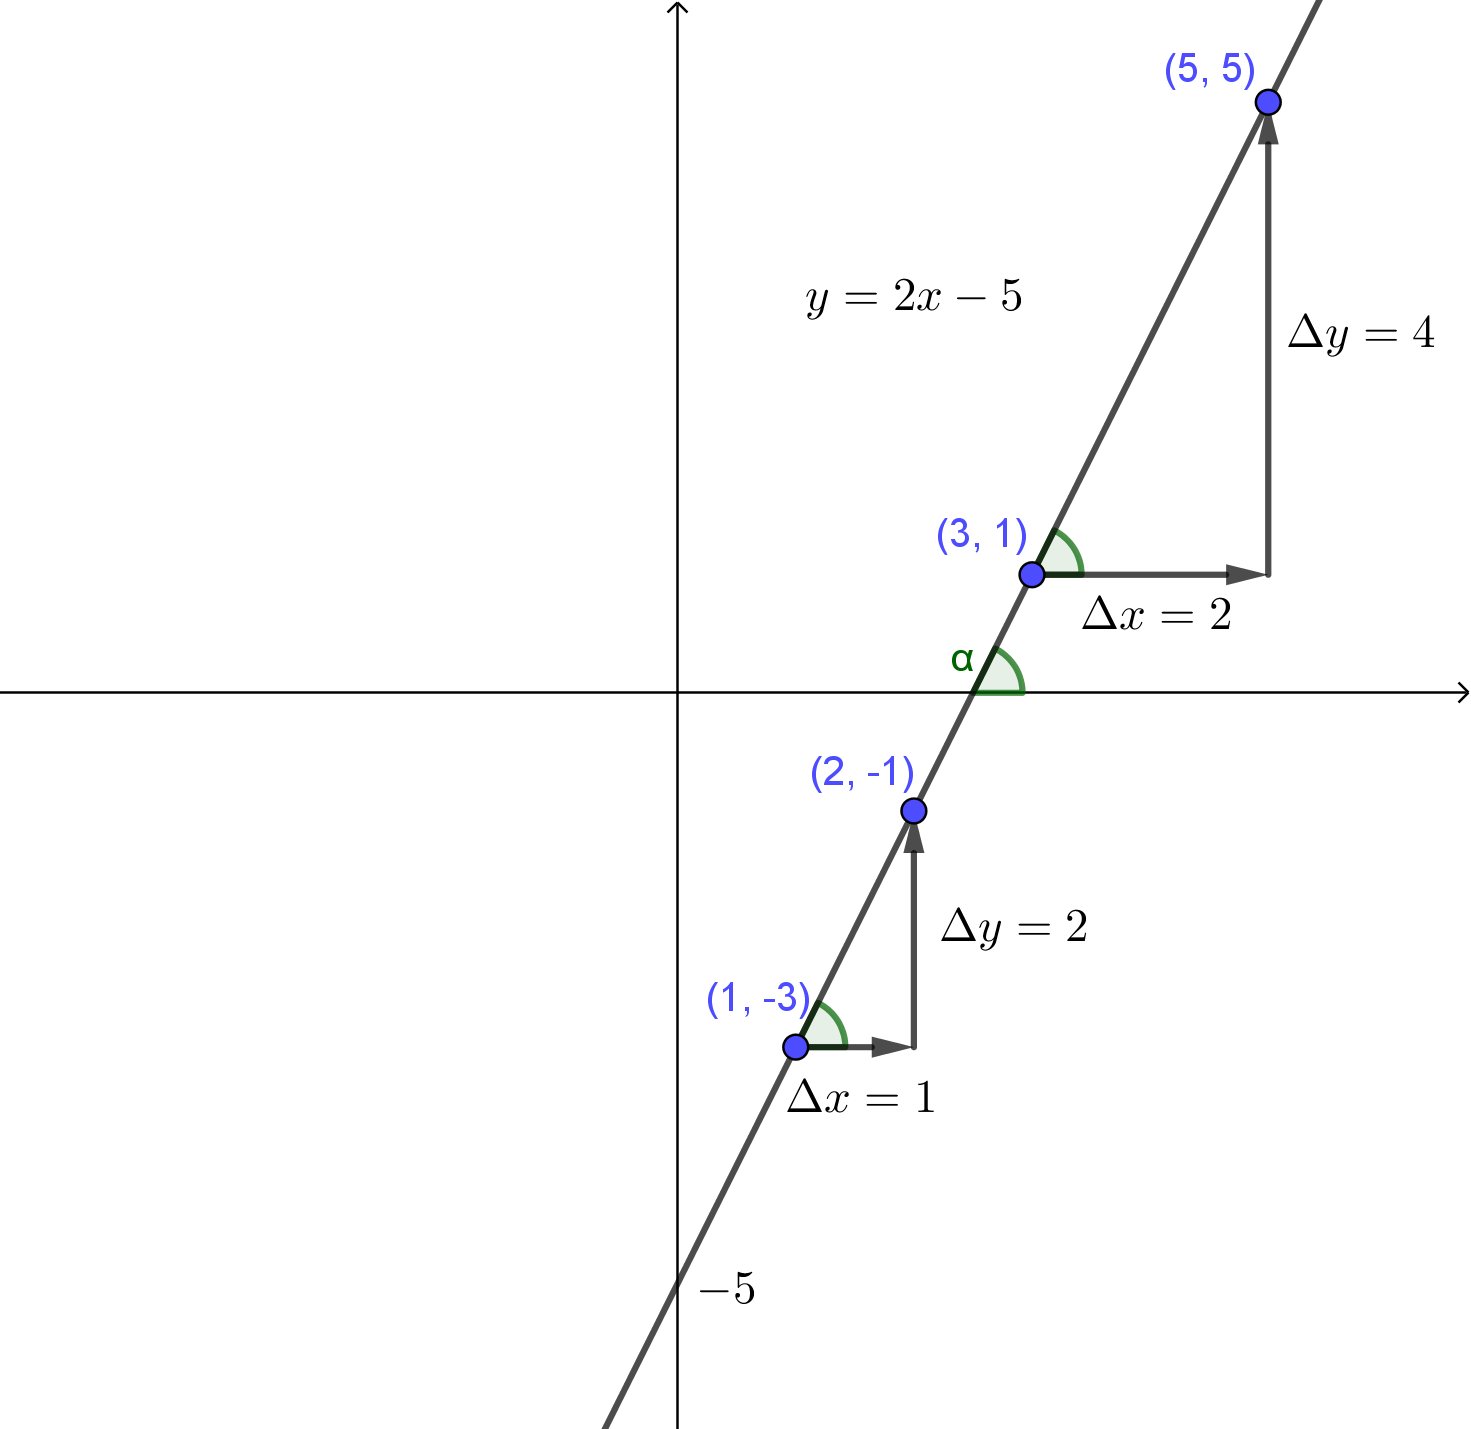
\includegraphics[width=0.7\textwidth]{line_1}
\end{center}

\clearpage
\bigskip\noindent\fbox{\(기울기=2\)}\par
\((1,-3)\)에서 \((2,-1)\)로의 변화를 살펴보면
\begin{gather*}
\Delta x=x\text{의 변화량}=2-1=1\\
\Delta y=y\text{의 변화량}=(-1)-(-3)=2
\end{gather*}
이므로
\[기울기=\frac{\Delta y}{\Delta x}=\frac21=2\]
이다.

\bigskip
\((3,1)\)에서 \((5,5)\)로의 변화를 살펴보아도
\begin{gather*}
\Delta x=5-3=2\\
\Delta y=5-1=4
\end{gather*}
이므로
\[기울기=\frac{\Delta y}{\Delta x}=\frac42=2\]
이다.

\bigskip
한편, 직선과 \(x\)축의 양의 방향이 이루는 각도를 \(\alpha\)라고 하면 \(\tan\alpha=\frac{\Delta y}{\Delta x}\)이므로
\[기울기=\tan\alpha\]
이기도 하다.

\bigskip\noindent\fbox{\(y절편=-1\)}\par
이 그래프가 \(y\)축과 만나는 점은 \((0,-5)\)이다.
따라서 \(y\)절편은 \(-5\)이다.
\clearpage
%line2
\prob{\(y=-\frac13x+3\)의 그래프를 그려보자.}\label{line2}
\vspace{-30pt}
\begin{align*}
x=-3&\longrightarrow y=4\\
x=0&\longrightarrow y=3\\
x=3&\longrightarrow y=\pb{2}\\
x=6&\longrightarrow y=\pb{1}\\
&\vdots
\end{align*}
따라서 이 그래프는 \((-3,4)\), \((0,3)\), \((3,\pb2)\), \((6,\pb1)\) 등을 지난다.

\begin{center}
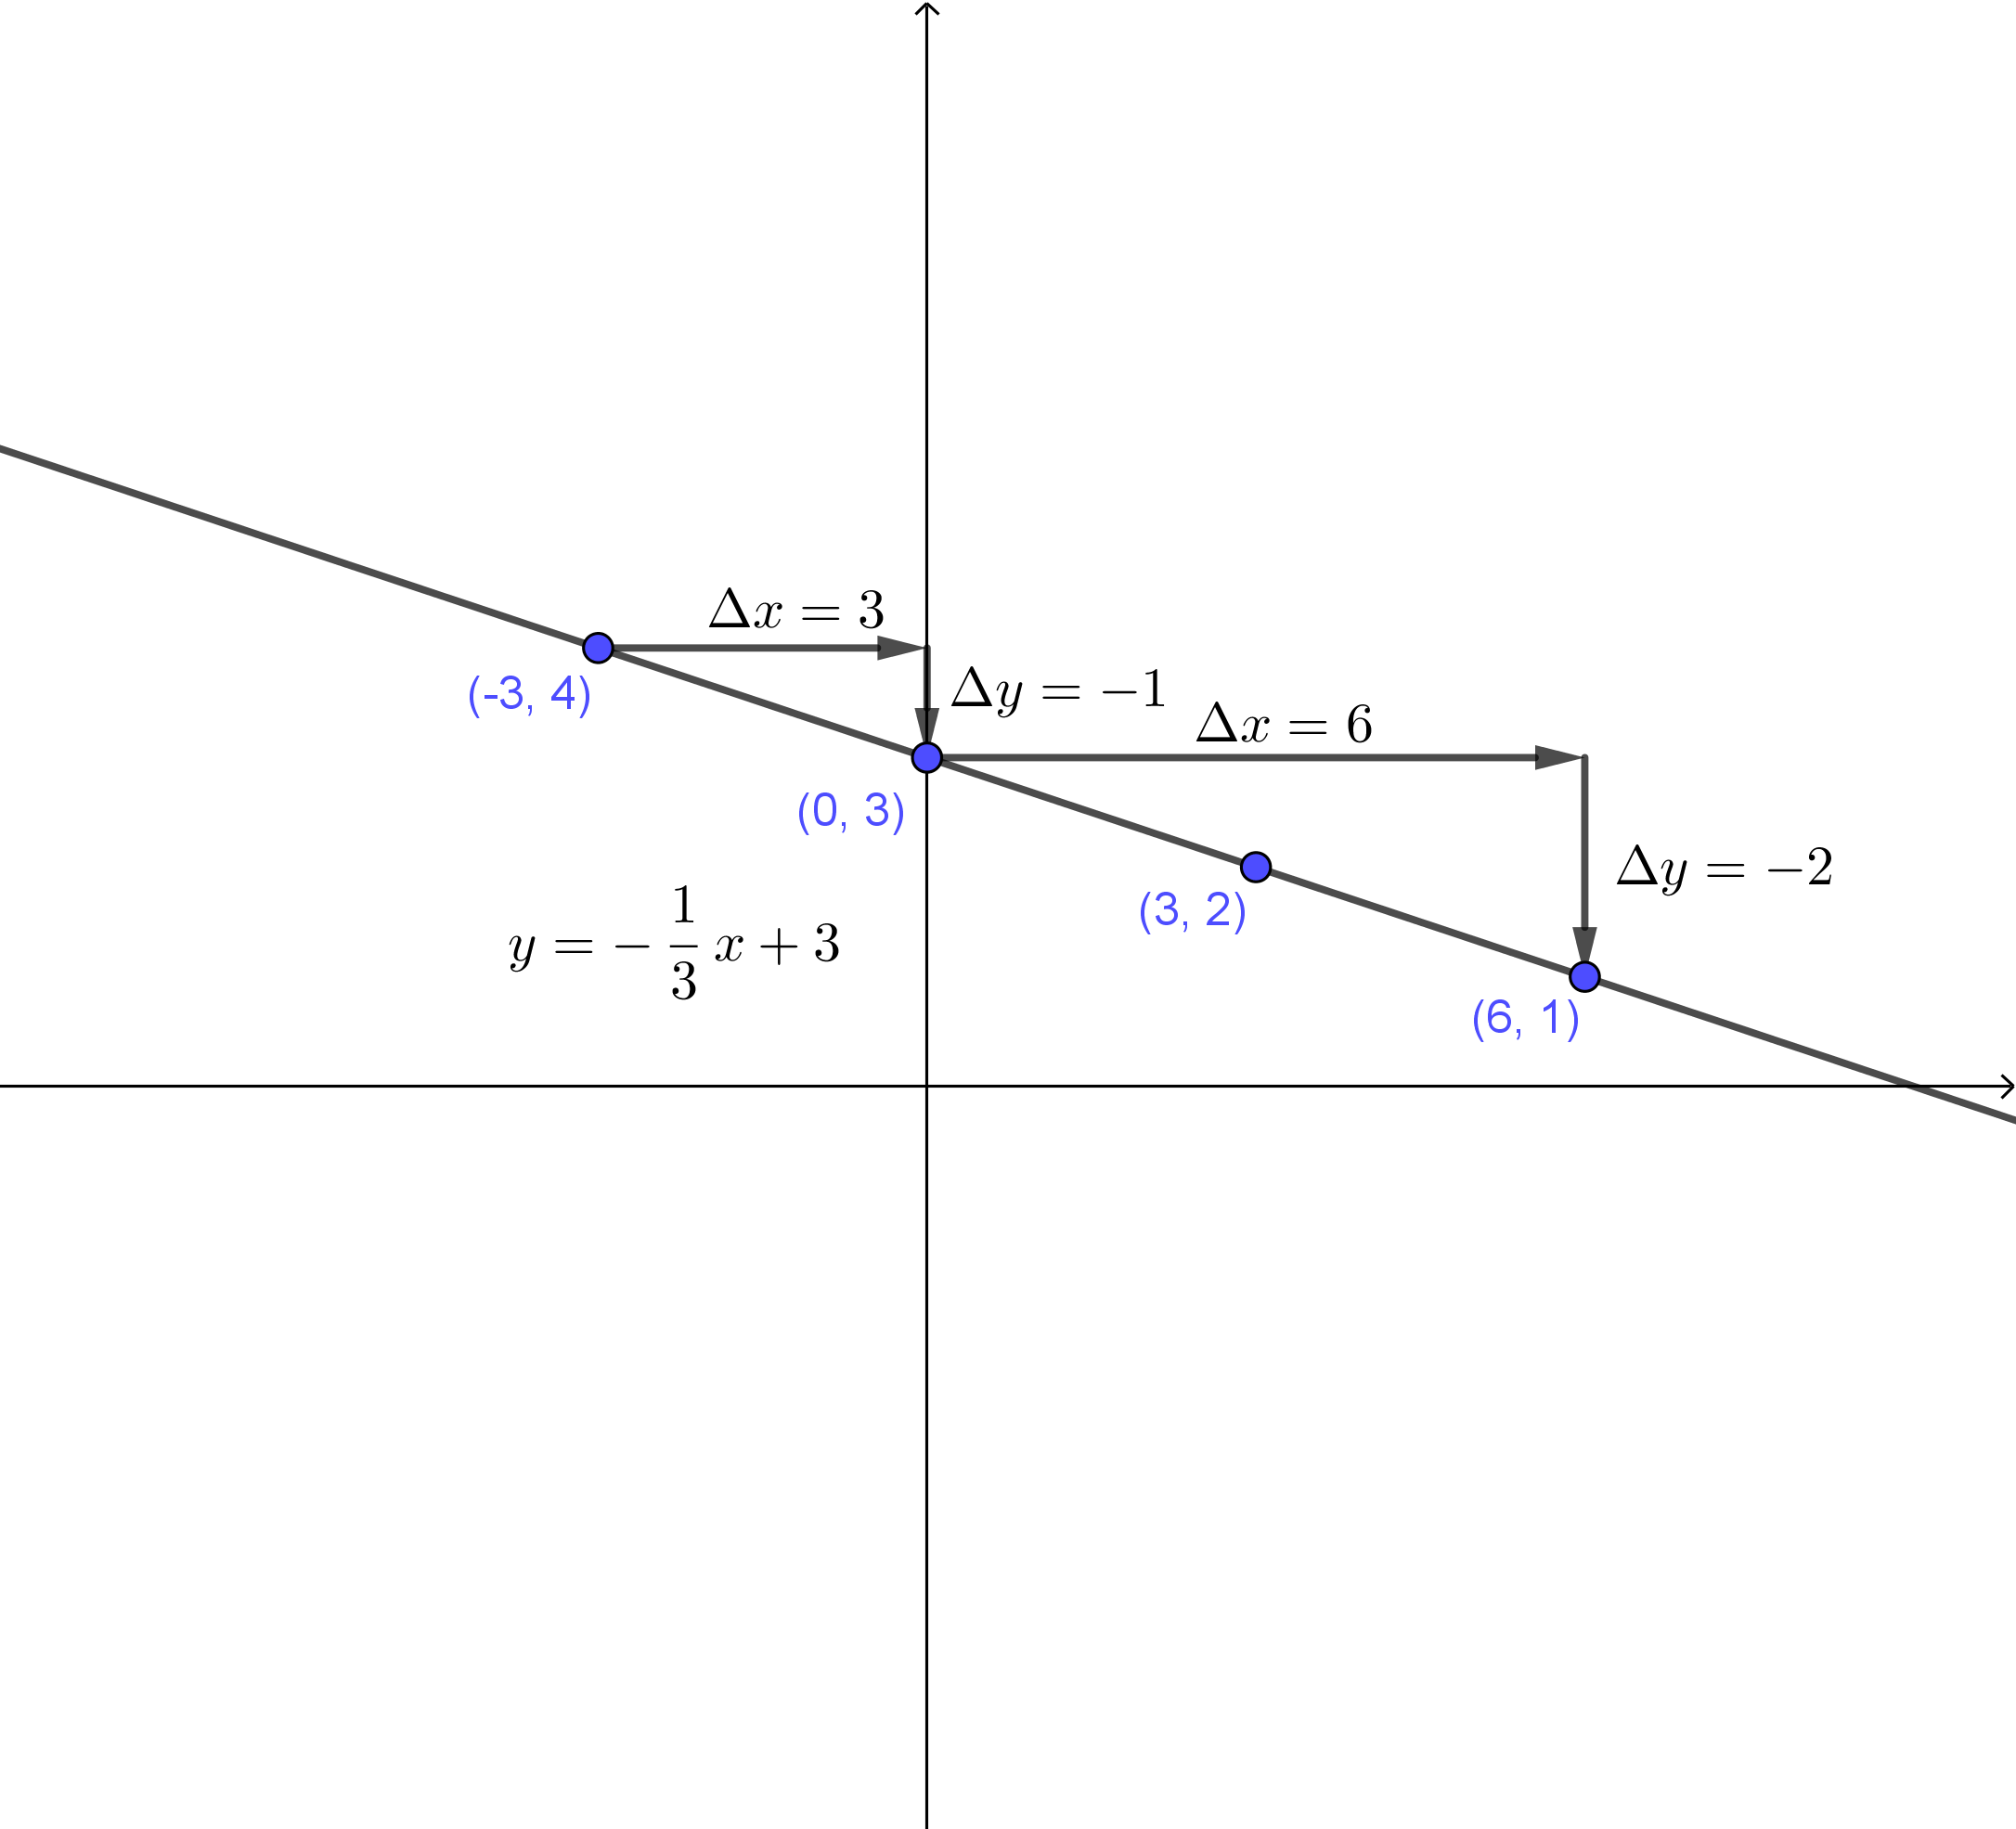
\includegraphics[width=0.7\textwidth]{line_2}
\end{center}
\bigskip\noindent\fbox{\(기울기=\pb{-\frac13}\)}\par
\((-3,4)\)에서 \((0,3)\)로의 변화를 살펴보면
\begin{gather*}
\Delta x=0-(-3)=3\\
\Delta y=3-4=-1\\
기울기=\frac{\Delta y}{\Delta x}=\pb{-\frac13}
\end{gather*}
이다.

\bigskip
\((0,3)\)에서 \((6,1)\)로의 변화를 살펴보아도 기울기의 값은 같다.
\begin{gather*}
\Delta x=6-0=6\\
\Delta y=1-3=-2\\
기울기=\frac{\Delta y}{\Delta x}=\pb{-\frac13}
\end{gather*}

\bigskip\noindent\fbox{\(y절편=\pb4\)}\par
이 그래프가 \(y\)축과 만나는 점은 \((0,\pb4)\)이다.
따라서 \(y\)절편은 \(\pb4\)이다.

\bigskip
%line3
\begin{mdframed}\label{line3}
\theo{\(y=mx+n\)의 그래프}
함수 \(y=mx+n\)의 그래프는 기울기가 \(m\)이고, \(y\)절편이 \(n\)인 직선이다.
이때,
\begin{itemize}
\item
기울기는 \:\(\frac{\Delta y}{\Delta x}\)\:을 의미한다.
(\(\Delta x=x\)의 변화량, \(\Delta y=y\)의 변화량)
\item
직선과 \(x\)축의 양의 방향이 이루는 각도를 \(\alpha\)라고 하면
\[기울기=\tan\alpha\]
이기도 하다.
(단, \(기울기>0\))
\item
\(y\)절편은 그래프가 \(y\)축과 만나는 점의 \(y\)좌표를 의미한다.
\end{itemize}
\end{mdframed}

%line4
\rema{}\label{line4}
예시 \ref{line1})와 문제 \ref{line2})에서, 단순히 기울기와 \(y\)절편을 가지고 그려도 된다.
\begin{enumerate}
\item
\(y=2x-5\)의 그래프를 그리려면 \((0,-5)\)에서부터 출발해 기울기가 \(2\)가 되도록 직선을 그리면 된다.
\item
\(y=-\frac13x+3\)의 그래프를 그리려면 \((0,-3)\)에서부터 출발해 기울기가 \(-\frac13\)이 되도록 직선을 그리면 된다.
\end{enumerate}

%line5
\prob{}\label{line5}
\(x\)축의 양의 방향과 \(60^\circ\)의 각도를 이루고 \(y\)절편이 \(1\)인 직선의 방정식을 구하여라.

%%lline
\section{직선의 방정식 \(ax+by+c=0\)}
%lline1
\exam{}\label{lline1}
\begin{enumerate}
\item
\(x+2y-4=0\)의 그래프를 그려보자.
(\(a=1\), \(b=2\), \(c=-4\))

이 식을 변형하면
\[y=-\frac12x+2\]
이 된다.
따라서 기울기가 \(-\frac12\)이고 \(y\)절편이 \(2\)인 직선이다.
\begin{center}
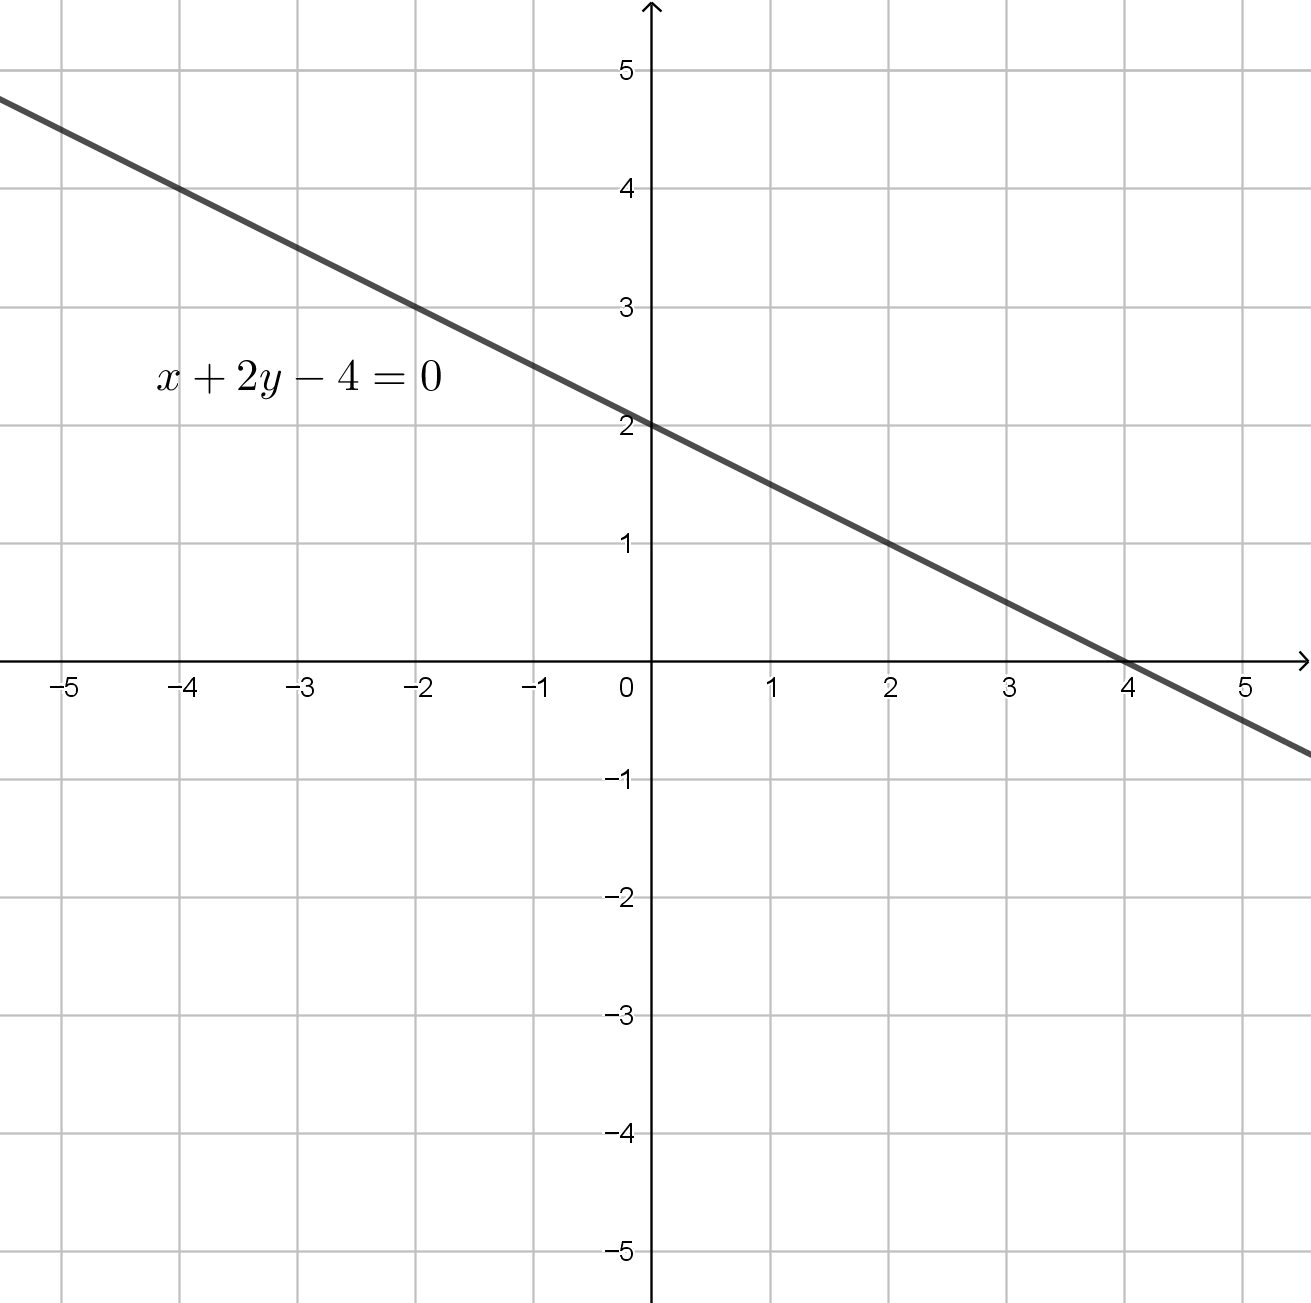
\includegraphics[width=0.5\textwidth]{line_3}
\end{center}
\item
\(y-3=0\)의 그래프를 그려보자.
(\(a=0\), \(b=1\), \(c=-3\))
\(y=3\)을 만족시키는 모든 점 \((x,y)\)를 찍으면 된다.
\[(-1,3),(0,3),(1,3),(2,3),\cdots\]
등을 잇는 직선을 그리면 다음과 같다.
\footnote{\(y=0x+3\)
로 해석하여 기울기가 \(0\)이고 \(y\)절편이 \(3\)인 직선을 그려도 된다.}
\begin{center}
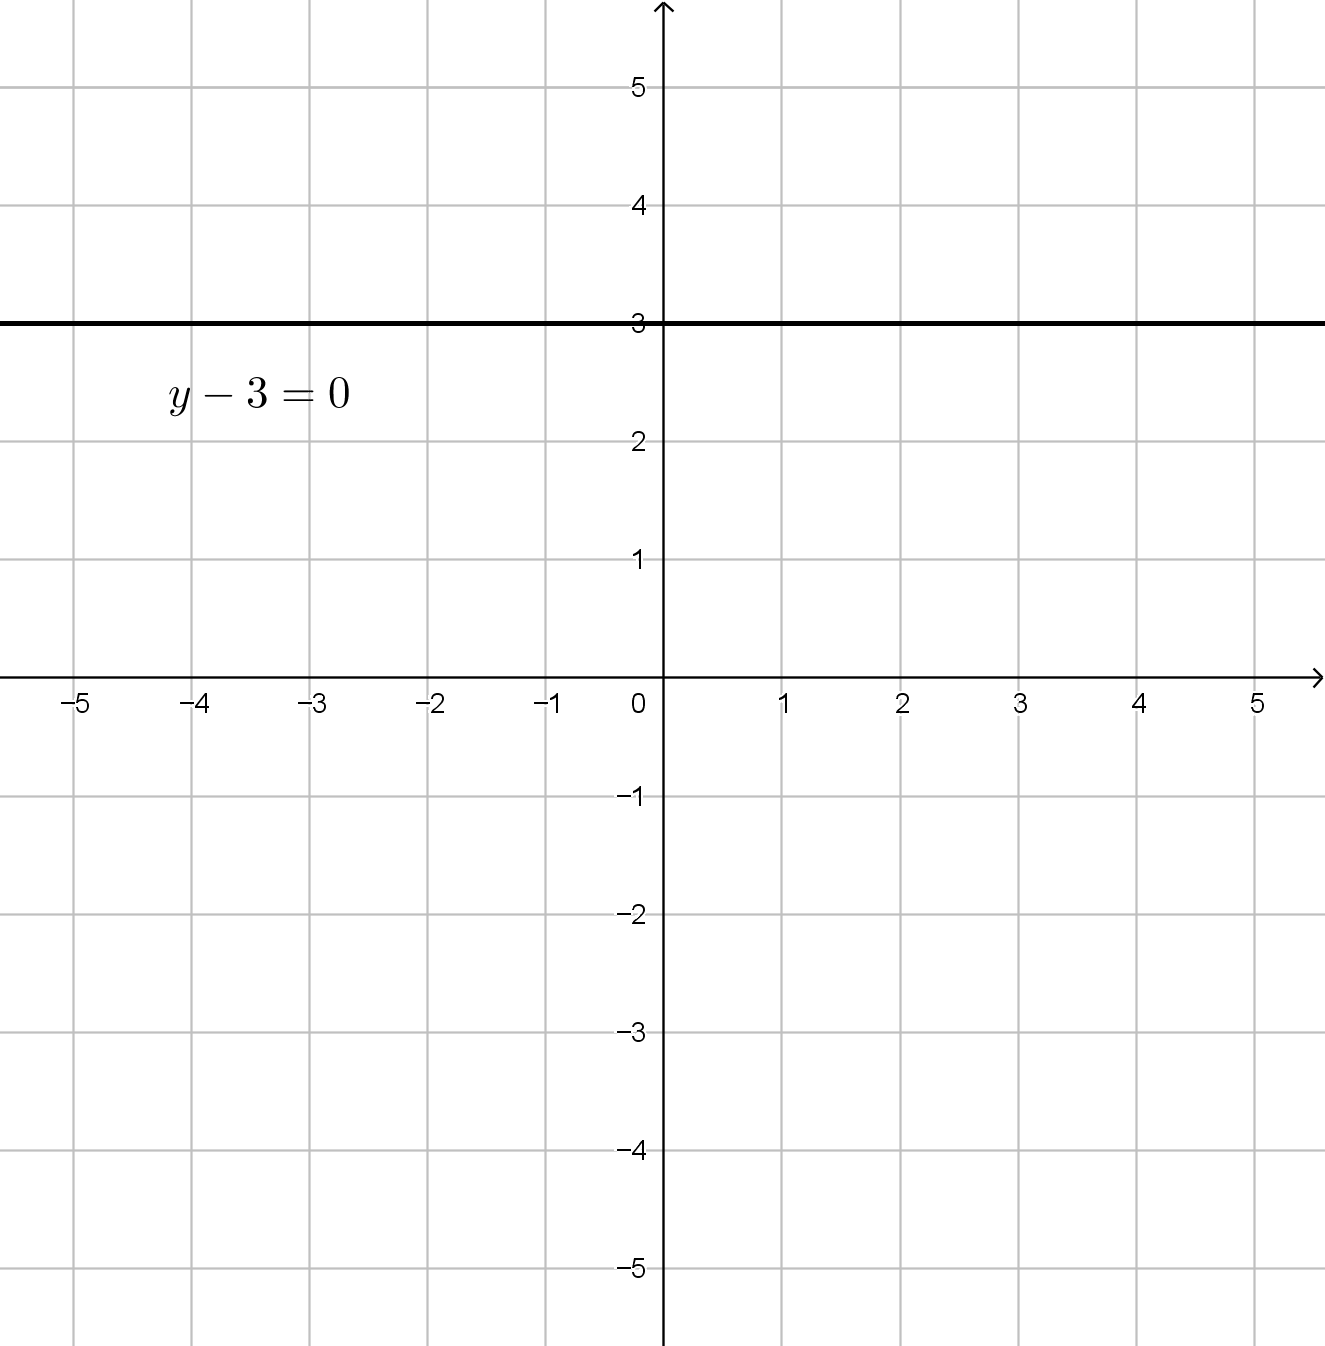
\includegraphics[width=0.5\textwidth]{line_4}
\end{center}
\item
\(x+1=0\)의 그래프를 그려보자.
(\(a=1\), \(b=0\), \(c=1\))

\(x=-1\)인 모든 점 \((x,y)\)들을 찍으면 다음 직선이 된다.
\begin{center}
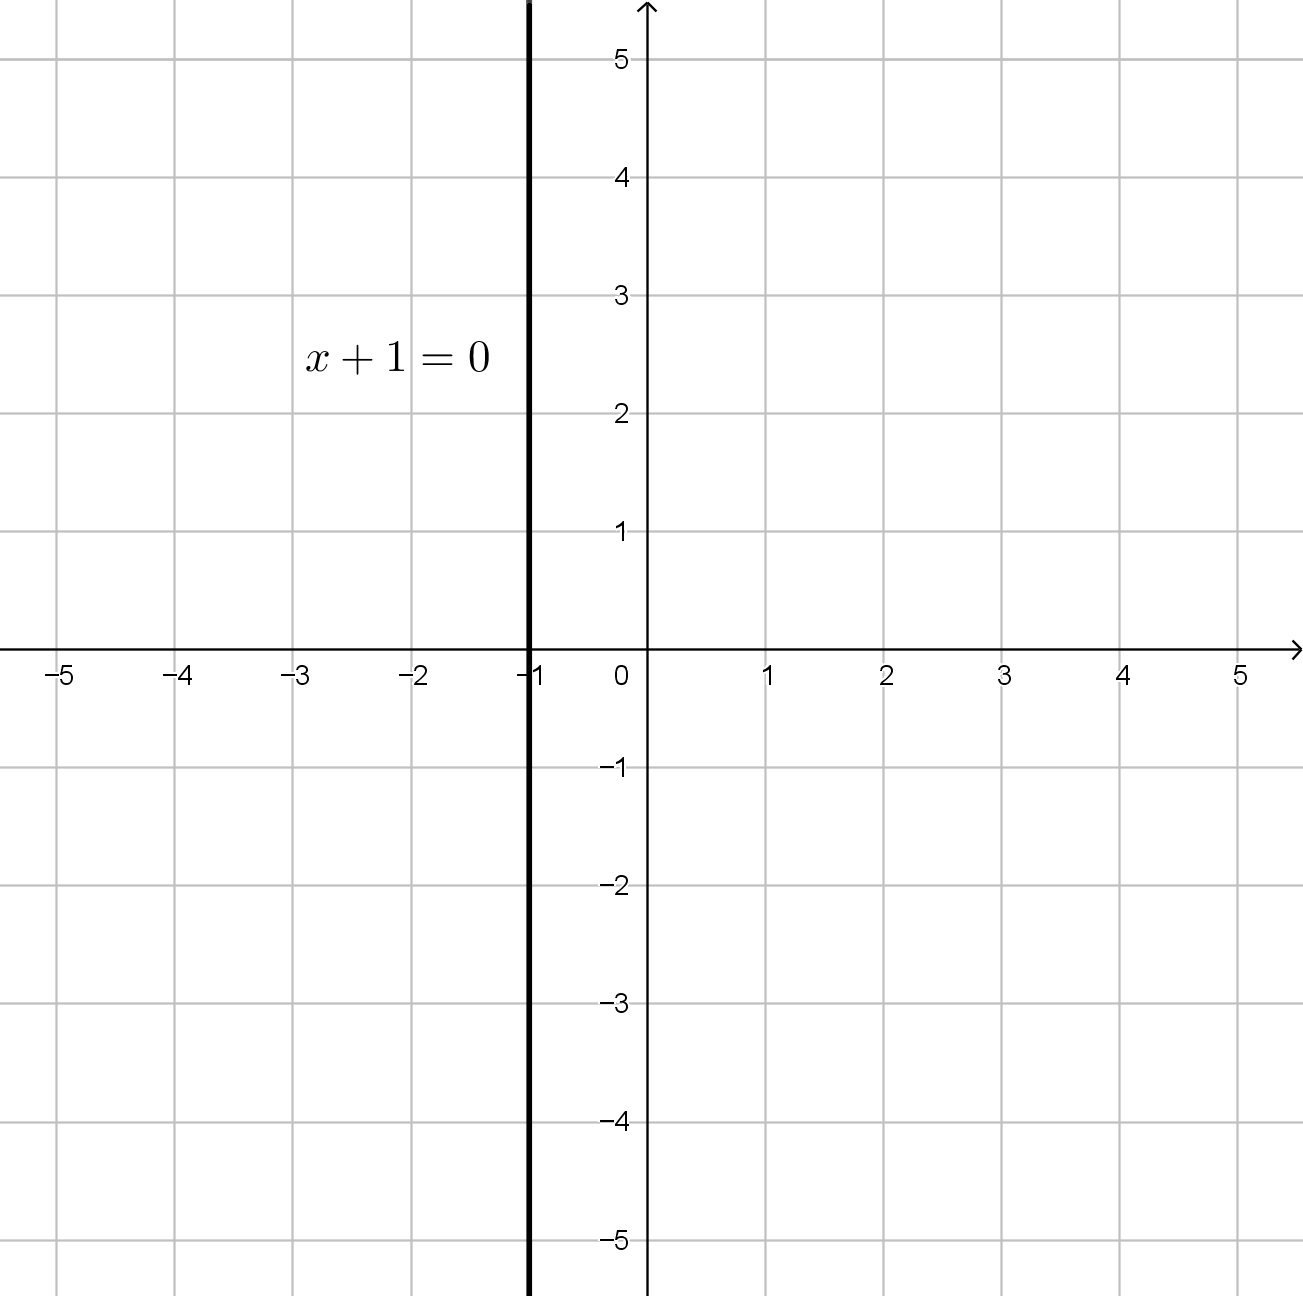
\includegraphics[width=0.5\textwidth]{line_5}
\end{center}
\end{enumerate}

%lline2
\begin{mdframed}
\theo{\(ax+by+c=0\)의 그래프}\label{lline2}
\(b=0\)인 경우 \(x=k\) 꼴로 변형시킬 수 있다.\\
\(a=0\)인 경우 \(y=k\) 꼴로 변형시킬 수 있다.
\begin{itemize}
\item
\(x=k\)의 그래프는 \(x\)절편이 \(k\)이고 \(y\)축과 평행한 직선이다.
\item
\(y=k\)의 그래프는 \(y\)절편이 \(k\)이고 \(x\)축과 평행한 직선이다.
\end{itemize}
\end{mdframed}

\clearpage
%lline3
\prob{다음 식들의 그래프를 그려라}\label{lline3}
\par\medskip
\begin{minipage}{0.45\textwidth}\centering
\(y=x+2\)
\par\bigskip\includegraphics[width=0.9\textwidth]{55}
\end{minipage}
\begin{minipage}{0.45\textwidth}\centering
\(y=3x-3\)
\par\bigskip\includegraphics[width=0.9\textwidth]{55}
\end{minipage}\bigskip\bigskip\par
\begin{minipage}{0.45\textwidth}\centering
\(y=-3x+5\)
\par\bigskip\includegraphics[width=0.9\textwidth]{55}
\end{minipage}
\begin{minipage}{0.45\textwidth}\centering
\(y=-2x\)
\par\bigskip\includegraphics[width=0.9\textwidth]{55}
\end{minipage}\bigskip\bigskip\par
\begin{minipage}{0.45\textwidth}\centering
\(y=\frac12x-2\)
\par\bigskip\includegraphics[width=0.9\textwidth]{55}
\end{minipage}
\begin{minipage}{0.45\textwidth}\centering
\(y=-\frac23x+1\)
\par\bigskip\includegraphics[width=0.9\textwidth]{55}
\end{minipage}\bigskip\bigskip\par

\clearpage
\begin{minipage}{0.45\textwidth}\centering
\(2x+y-1=0\)
\par\bigskip\includegraphics[width=0.9\textwidth]{55}
\end{minipage}
\begin{minipage}{0.45\textwidth}\centering
\(2x+3y+6=0\)
\par\bigskip\includegraphics[width=0.9\textwidth]{55}
\end{minipage}\bigskip\bigskip\par
\begin{minipage}{0.45\textwidth}\centering
\(x+y=2\)
\par\bigskip\includegraphics[width=0.9\textwidth]{55}
\end{minipage}
\begin{minipage}{0.45\textwidth}\centering
\(y=-1\)
\par\bigskip\includegraphics[width=0.9\textwidth]{55}
\end{minipage}\bigskip\bigskip\par
\begin{minipage}{0.45\textwidth}\centering
\(x=-1\)
\par\bigskip\includegraphics[width=0.9\textwidth]{55}
\end{minipage}
\begin{minipage}{0.45\textwidth}\centering
\(x=0\)
\par\bigskip\includegraphics[width=0.9\textwidth]{55}
\end{minipage}\bigskip\bigskip\par

%%two
\section{두 직선의 위치관계}
평면 위에 두 직선이 있다면 다음의 세 경우 중 하나이다.
\par\bigskip\noindent
\begin{tabu}{X[2,c]|X[2,c]|X[2,c]}
\toprule
일치한다	&평행하다	&한 점에서 만난다\\
\hline
 \raisebox{-.5\height}{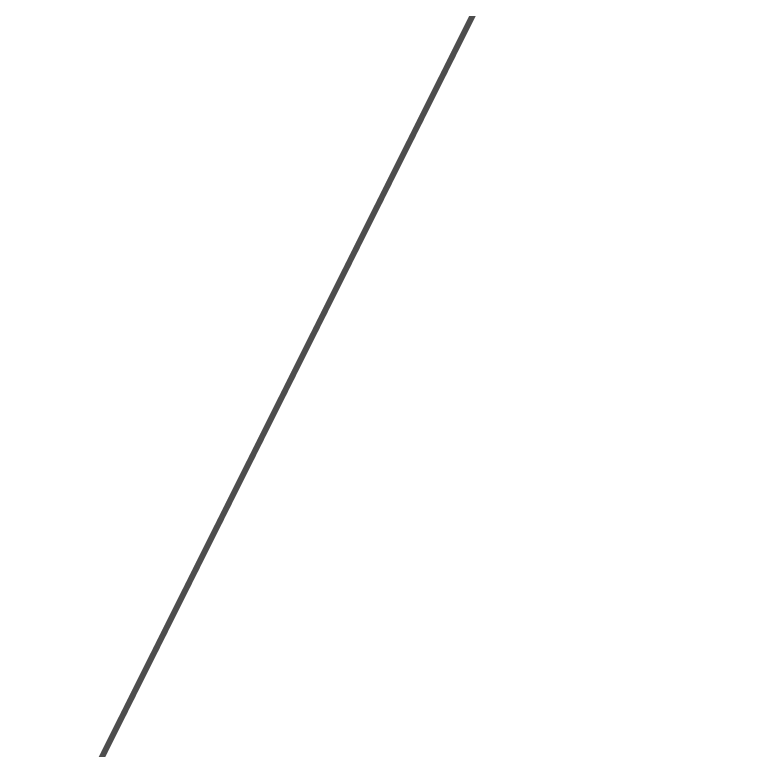
\includegraphics[width=0.24\textwidth]{twolines_1}}
&\raisebox{-.5\height}{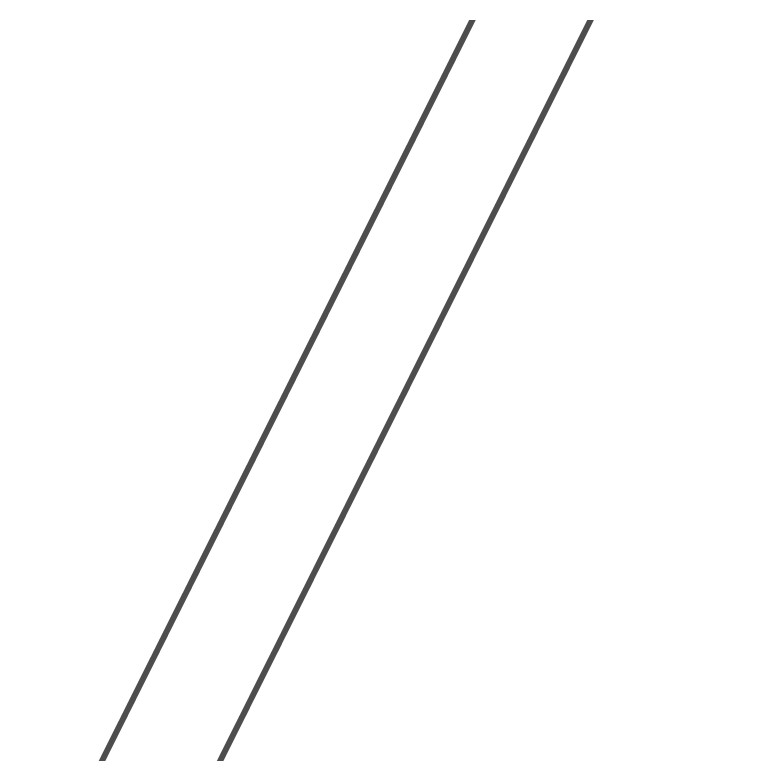
\includegraphics[width=0.24\textwidth]{twolines_2}}
&\raisebox{-.5\height}{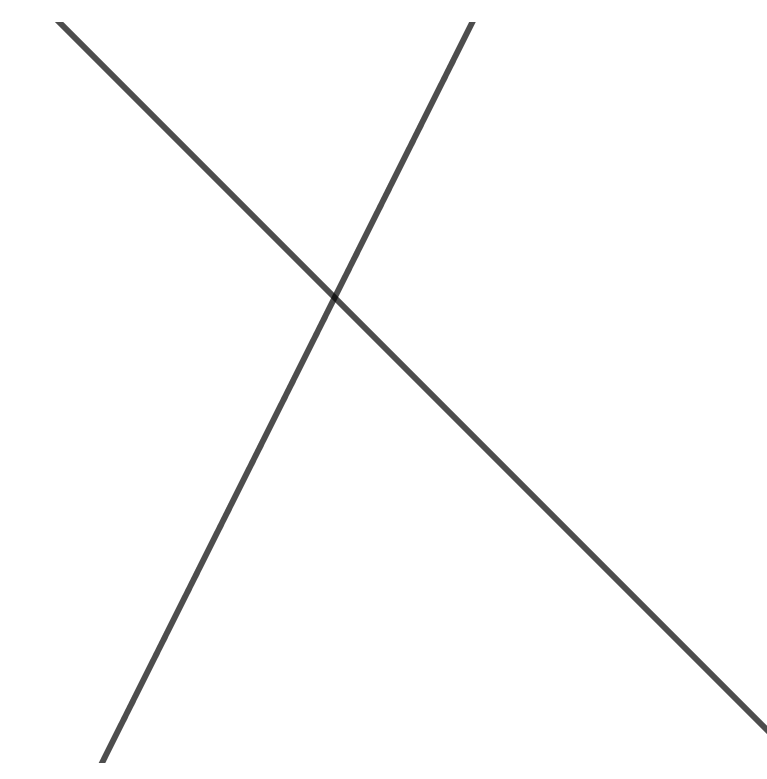
\includegraphics[width=0.24\textwidth]{twolines_3}}
\\\bottomrule
\end{tabu}
\par\bigskip
이 위치관계는 두 직선의 기울기와 \(y\)절편에 의해 결정된다.

\begin{enumerate}
\item
두 직선이 \(y=mx+n\)과 \(y=m'x+n'\)일 때\\
\(m\)과 \(m'\)은 기울기, \(n\)과 \(n'\)은 \(y\)절편을 나타내므로,
\bigskip
\begin{center}
\begin{forest}
  for tree={grow'=east,calign = first,
    child anchor=west,
    l sep=10mm,
    s sep=5mm,
    anchor=east,
    align=center,draw,
    child anchor=parent,
    parent anchor=children,
    where level={1}{rounded corners}{},
    where level={2}{rounded corners}{},
    where level={3}{rounded corners}{},
    edge+={rounded corners=5pt, -{Stealth[length=10pt]}, line width=1pt},
  },
[{$y=mx+n$}\\
{$y=m'x+n'$},
  [{$m=m'$}
    [{$n=n'$}
      [일치,tier=word]
    ]
    [{$n\neq n'$},
    edge path={\noexpand\path[\forestoption{edge}] (!u.parent anchor) --+(5mm,0)
    |-(.child anchor)\forestoption{edge label};}
     [평행,tier=word]]
    ]
  [{$m\neq m'$},
    edge path={\noexpand\path[\forestoption{edge}] (!u.parent anchor) --+(5mm,0)
    |-(.child anchor)\forestoption{edge label};}
    [{한 점에서 만남},tier=word,rounded corners=0pt]
  ]
]
\end{forest}
\end{center}
\bigskip
\begin{mdframed}
%two1
\theo{}\label{two1}
두 직선 \(y=mx+n\)과 \(y=m'x+n'\)은
\begin{itemize}
\item
\(m=m'\), \(n=n'\)이면 두 직선은 일치한다.
\item
\(m=m'\), \(n\neq n'\)이면 두 직선은 평행하다.
\item
\(m\neq m'\)이면 두 직선은 한 점에서 만난다.
\end{itemize}
\end{mdframed}
\item
한편, 두 직선이 \(ax+by+c=0\), \(a'x+b'y+c'=0\)일 때,
\begin{gather*}
y=-\frac abx-\frac cb\\
y=-\frac{a'}{b'}x-\frac{c'}{b'}
\end{gather*}
으로부터
기울기가 같으려면
\(\frac ab=\frac{a'}{b'}\)이어야 한다.
즉
\[\frac a{a'}=\frac b{b'}\]
이면 된다.
또 \(y\)절편이 같으려면
\(\frac cb=\frac{c'}{b'}\)이어야 한다.
즉
\[\frac b{b'}=\frac c{c'}\]
이면 된다. 따라서
\bigskip
\begin{center}
\begin{forest}
  for tree={grow'=east,calign = first,
    child anchor=west,
    l sep=10mm,
    s sep=5mm,
    anchor=east,
    align=center,draw,
    child anchor=parent,
    parent anchor=children,
    where level={1}{rounded corners}{},
    where level={2}{rounded corners}{},
    where level={3}{rounded corners}{},
    edge+={rounded corners=5pt, -{Stealth[length=10pt]}, line width=1pt},
  },
[{$ax+by+c=0$}\\
{$a'x+b'y+c'=0$},
  [{$\displaystyle\frac{a}{b}=\frac{a'}{b'}$}
    [{$\displaystyle\frac{b}{b'}=\frac{c}{c'}$}
      [일치,tier=word]
    ]
    [{$\displaystyle\frac{b}{b'}\ne\frac{c}{c'}$},
    edge path={\noexpand\path[\forestoption{edge}] (!u.parent anchor) --+(5mm,0)
    |-(.child anchor)\forestoption{edge label};}
     [평행,tier=word]]
    ]
  [{$\displaystyle\frac{a}{b}\ne\frac{a'}{b'}$},
    edge path={\noexpand\path[\forestoption{edge}] (!u.parent anchor) --+(5mm,0)
    |-(.child anchor)\forestoption{edge label};}
    [{한 점에서 만남},tier=word,rounded corners=0pt]
  ]
]
\end{forest}
\end{center}
\bigskip

\begin{mdframed}
%two2
\theo{}\label{two2}
두 직선 \(ax+by+c=0\)과 \(a'x+b'y+c'=0\)은
\begin{itemize}
\item
\(\frac{a}{a'}=\frac{b}{b'}=\frac{c}{c'}\)이면 두 직선은 일치한다.
\item
\(\frac{a}{a'}=\frac{b}{b'}\neq\frac{c}{c'}\)이면 두 직선은 평행하다.
\item
\(\frac{a}{a'}\neq\frac{b}{b'}\)이면 두 직선은 한 점에서 만난다.
\end{itemize}
\end{mdframed}
\end{enumerate}

\clearpage
%two3
\prob{}\label{two3}
두 직선 \(y=-2x+5\), \(y=(a-2)x+3\)이 서로 평행하기 위한 \(a\)의 값을 구하여라.
\bigskip

%two4
\prob{}\label{two4}
두 직선 \(y=ax-2\), \(y=(6-2a)x+1\)이 한 점에서 만나기 위한 \(a\)의 조건을 구하여라.
\bigskip

%two5
\prob{}\label{two5}
두 직선 \(ax+2y+3=0\), \(2x+(5-a)y+6=0\)이 서로 일치하기 위한 \(a\)의 값을 \(a_1\), 서로 평행하기 위한 \(a\)의 값을 \(a_2\)라고 할 때, \(a_2-a_1\)의 값을 구하여라.
\bigskip

%two6
\prob{}\label{two6}
연립방정식
\[
\begin{cases}
x+y+3=0\\
ax-3y+2=0
\end{cases}
\]
의 해가 존재하지 않을 때 \(a\)의 값을 구하여라.
\bigskip

%two7
\prob{}\label{two7}
연립방정식
\[
\begin{cases}
ax+6y-2=0\\
x-3y+b=0
\end{cases}
\]
의 해가 무수히 많을 때 \(a+b\)의 값을 구하여라.

\clearpage
두 직선이 한 점에서 만나는 경우 중 서로 수직인 경우가 있을 수 있다.
\begin{center}
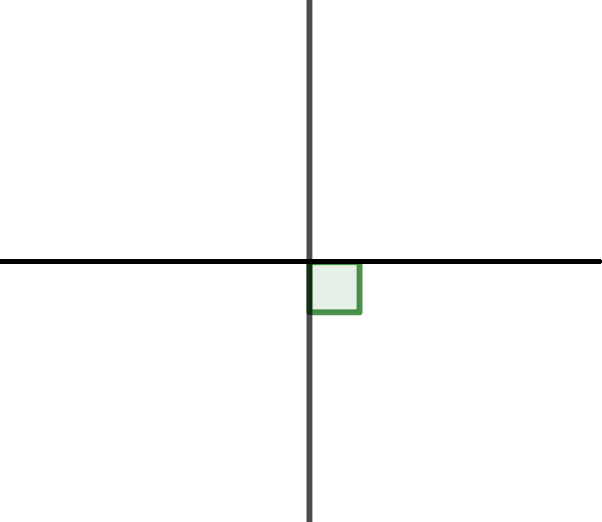
\includegraphics[width=0.3\textwidth]{perp_01}
~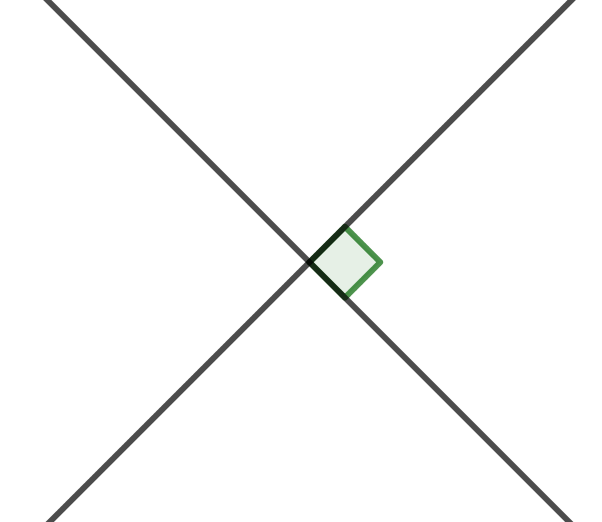
\includegraphics[width=0.3\textwidth]{perp_02}
~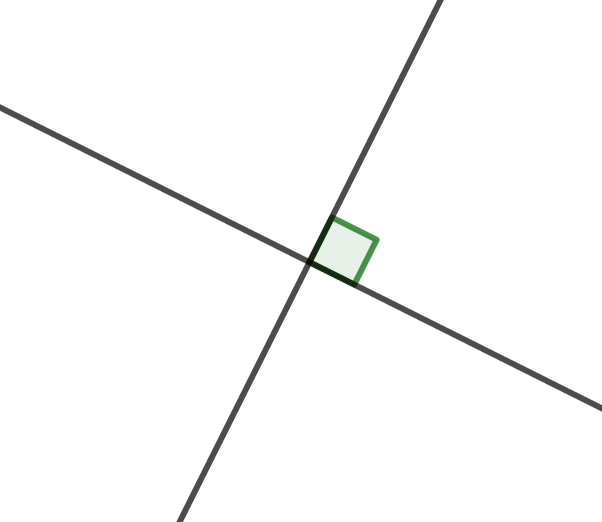
\includegraphics[width=0.3\textwidth]{perp_03}
\end{center}

%two8
\exam{}\label{two8}
좌표평면 위에 \(A(1,2)\), \(B(1,0)\), \(C(2,0)\), \(D(2,-1)\)을 생각하자.
\begin{center}
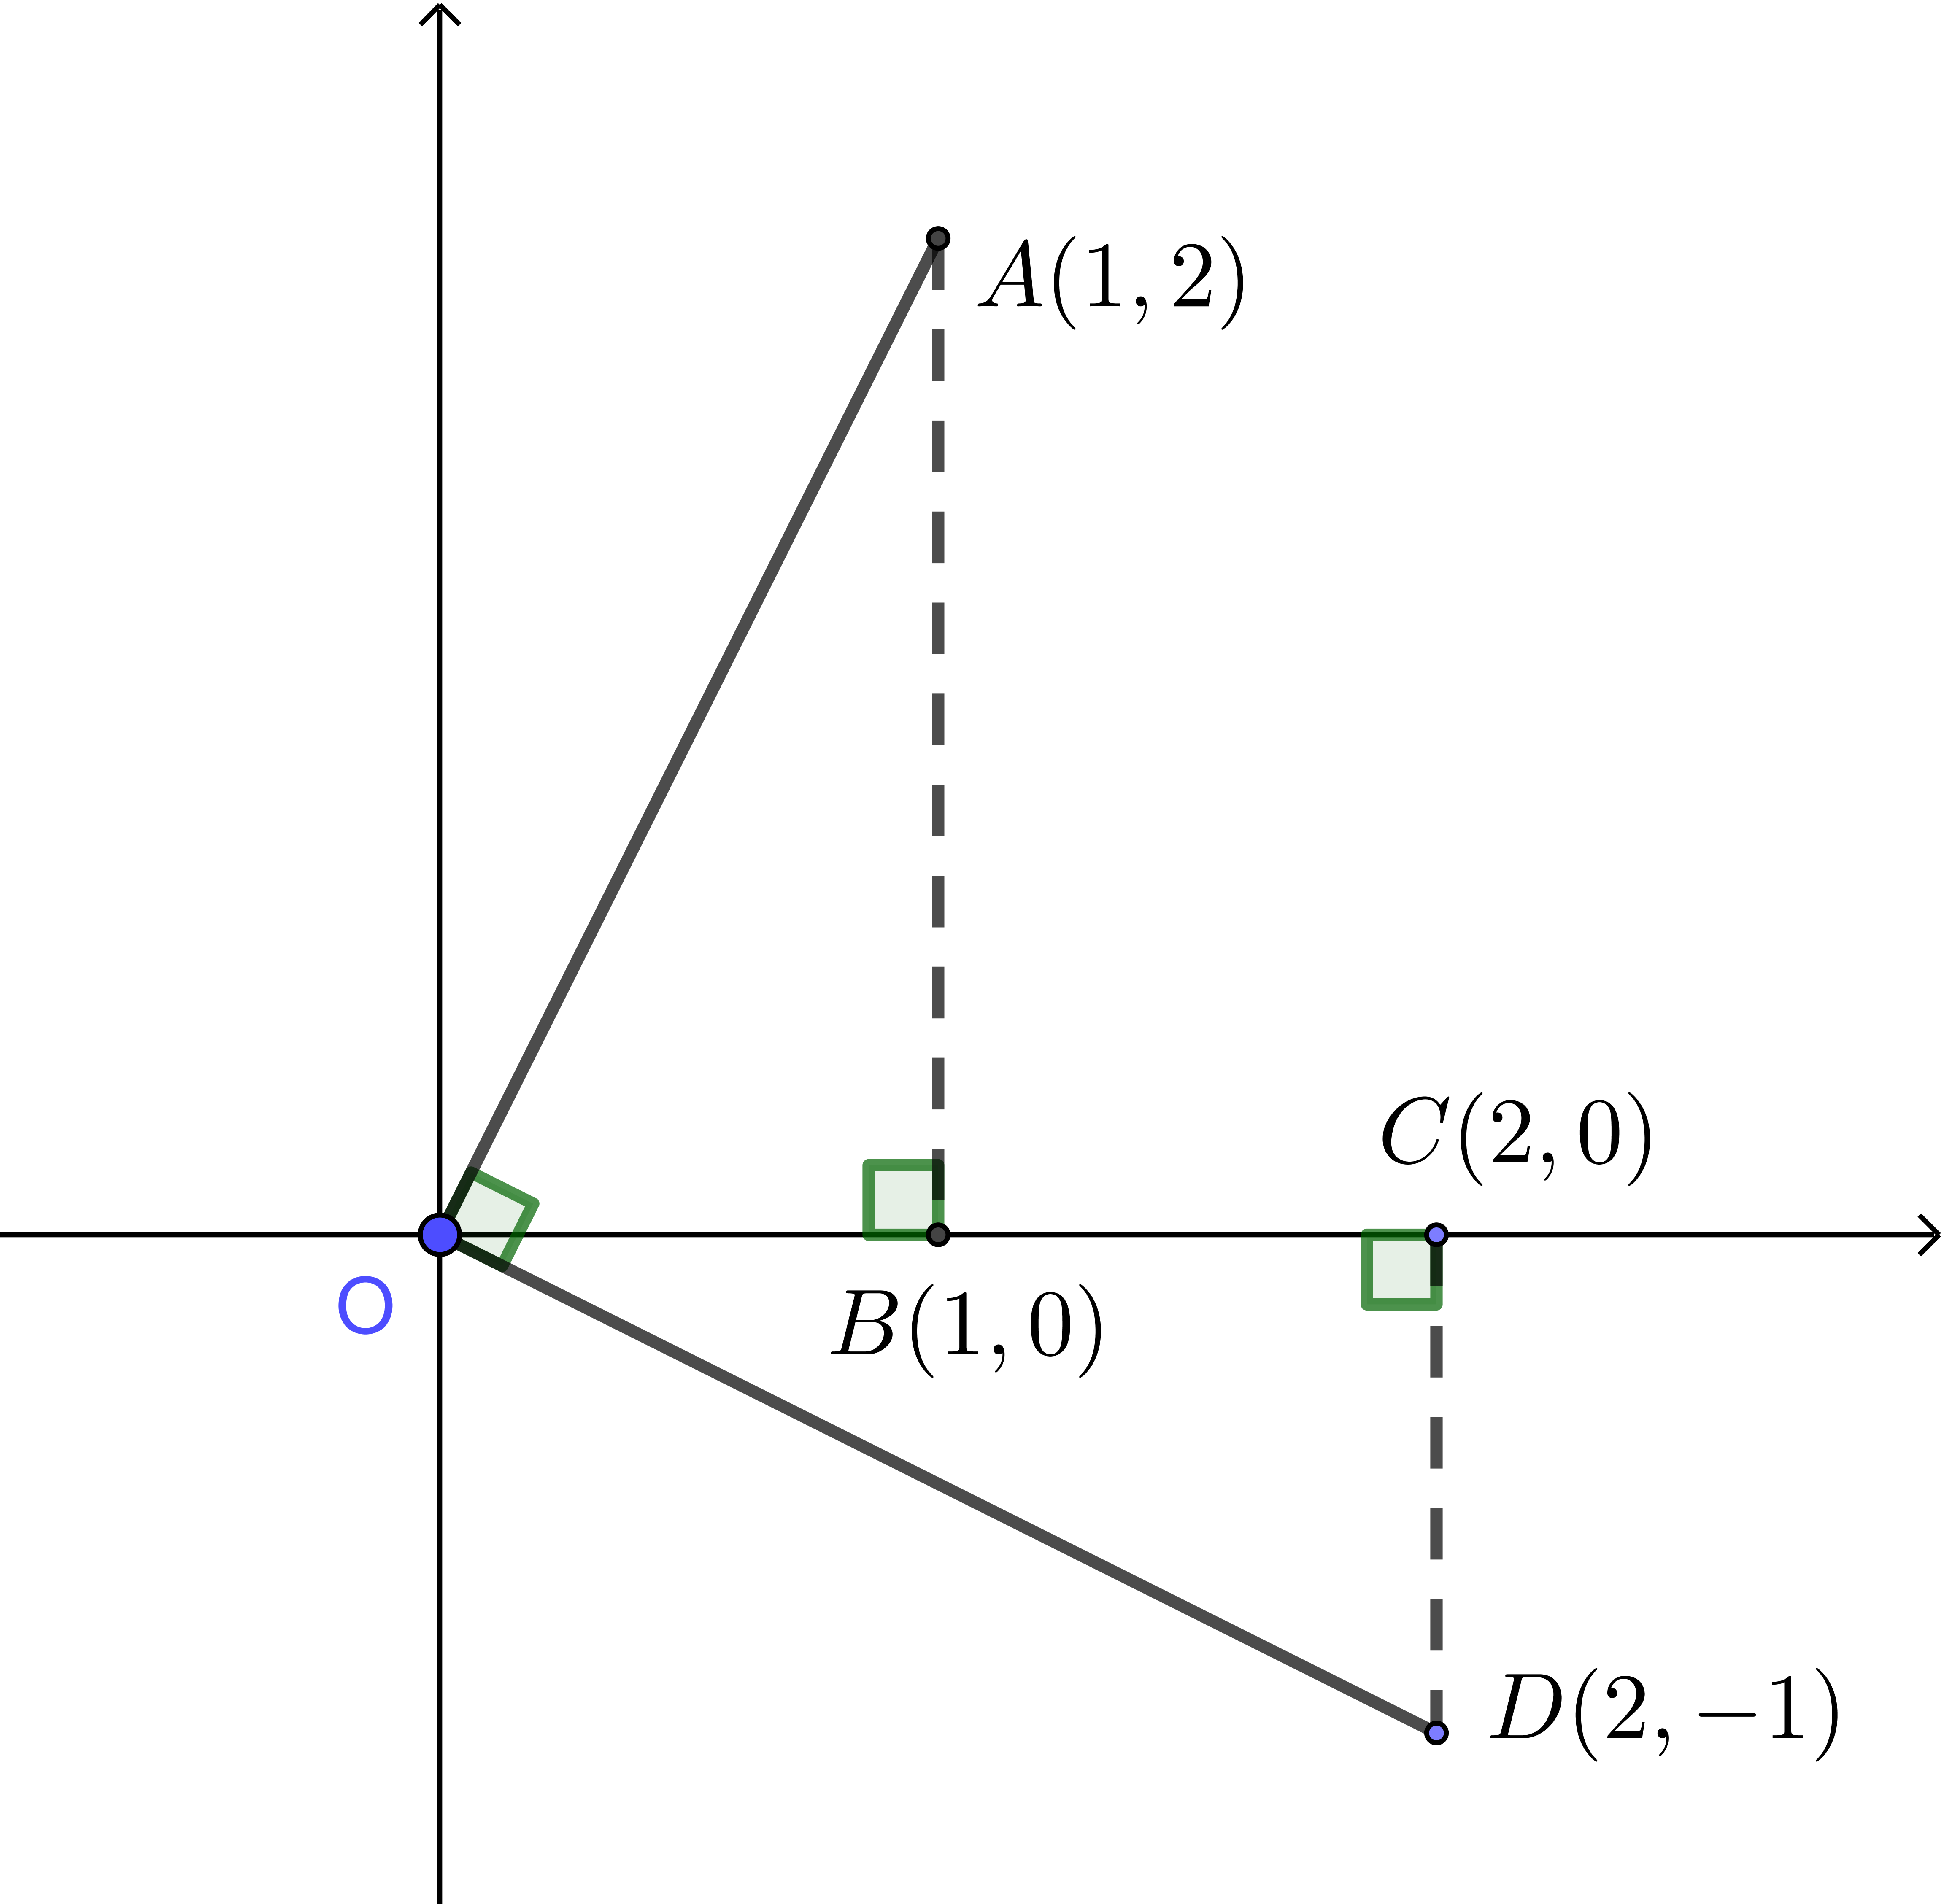
\includegraphics[width=0.35\textwidth]{twolines_7}
\end{center}
그러면
\[\triangle AOB\equiv\triangle DOC(SSS합동)\]
따라서
\begin{align*}
\angle AOD
&=\angle AOB+\angle DOC\\
&=\angle AOB+\angle OCB\\
&=90^\circ
\end{align*}
\(\ov OA\)의 기울기는 \(2\)이고, \(\ov OD\)의 기울기는 \(-\frac12\)이므로
\begin{center}
\fbox{기울기가 \(2\)와 \(-\frac12\)인 두 직선은 서로 수직이다.}
\end{center}

\begin{mdframed}
%two9
\theo{두 직선이 서로 수직일(직교할) 조건}\label{two9}
\begin{enumerate}
\item
두 직선 \(y=mx+n\), \(y=m'x+n'\)이 수직이면 \(mm'=-1\)이다.
\item
두 직선 \(ax+by+c=0\), \(a'x+b'y+c'=0\)이 수직이면 \(aa'+bb'=0\)이다.
\end{enumerate}
\end{mdframed}
\proo
\begin{enumerate}
\item
기울기가 같으면 방향도 같으므로, \(y=mx\)와 \(y=m'x\)가 수직일 조건을 구해도 된다.
따라서 두 직선 \(y=mx\)와 \(y=m'x\)를 고려하자.

\begin{center}
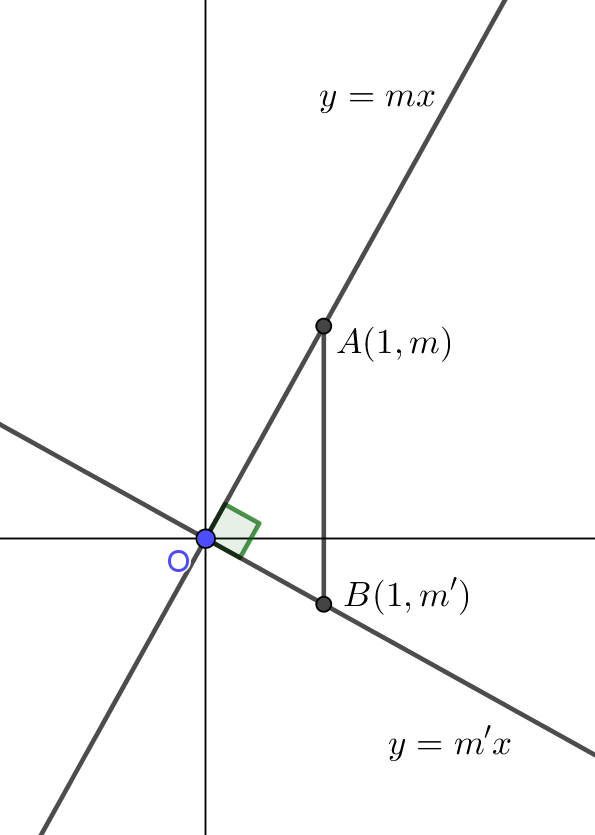
\includegraphics[width=0.3\textwidth]{twolines_8}
\end{center}

두 직선 위의 점 \(A(1,m)\), \(B(1,m')\)을 잡으면, \(\angle AOB=90^\circ\)이고 \(O=(0,0)\)이므로 피타고라스의 정리에 의해,
\[\ov OA^2+\ov OB^2=\ov AB^2\]
에서
\begin{gather*}
(1+m^2)+(1+m'^2)=(m-m')^2\\
m^2+m'^2+2=m^2-2mm'+m'^2\\
2=-2mm'\\
mm'=-1
\end{gather*}
\item
두 직선의 기울기는 각각
\(-\frac ab\), \(-\frac{a'}{b'}\)이므로%\footnotemark
\begin{gather*}
\left(-\frac ab\right)\left(-\frac{a'}{b'}\right)=-1\\
\frac ab\times\frac{a'}{b'}=-1\\
aa'=-bb'\\
aa'+bb'=0
\end{gather*}
\end{enumerate}
\qed

%two10
\prob{}\label{two10}
두 직선 \(y=-3x+5\)와 \(y=(a+1)x-1\)이 서로 수직할 때, \(a\)의 값을 구하여라.

\bigskip\bigskip
%two11
\prob{}\label{two11}
두 직선 \(y=(a+2)x+1\), \(y=(a-2)x-2\)이 서로 수직할 때, 가능한 모든 \(a\)값의 곱을 구하여라.

\bigskip\bigskip
%two12
\prob{}\label{two12}
두 직선 \(y=(a+3)x-1\), \(y=\left(a+\frac12\right)x+4\)이 \((2,3)\)에서 수직으로 만날 때 \(a\)의 값을 구하여라.

\bigskip\bigskip
%two13
\prob{}\label{two13}
두 직선 \(3x+(a+4)y+4=0\), \(ax-2y-3=0\)가 서로 수직할 때, \(a\)의 값을 구하여라.

%%three
\section{세 가지 공식}

%three1
\exam{기울기가 \(2\)이고 점 \(A(4,5)\)을 지나는 직선의 방정식을 구하여라.}\label{three1}
\begin{mdframed}
기울기가 \(2\)인 직선은 \(y=2x+n\)으로 표현될 수 있다.
이 직선이 \(A(4,5)\)을 지나므로,
\[5=2\cdot4+n\]
\(n=-3\)이다.
따라서 우리가 구하는 직선은
\[y=2x-3\]
이다.
\end{mdframed}

%three2
\prob{기울기가 \(\frac12\)이고 점 \(A(-2,3)\)를 지나는 직선의 방정식을 구하여라.}\label{three2}
\procedure{0.4}

\clearpage
\begin{mdframed}
%three3
\theo{}\label{three3}
기울기가 \(m\)이고 \(A(x_1,y_1)\)을 지나는 직선의 방정식은
\[y=m(x-x_1)+y_1\]
이다.
\end{mdframed}

\proo
기울기가 \(m\)인 직선은 \(y=mx+n\)으로 표현될 수 있다.
이 직선이 \(A(x_1,y_1)\)을 지나므로,
\[y_1=mx_1+n\]
\[n=-mx_1+y_1\]
이다.
따라서 우리가 구하는 직선은
\[y=mx-mx_1+y_1\]
\[y=m(x-x_1)+y_1\]
이다.
\qed

%three4
\exam{}\label{three4}
예시 \ref{three1})\을 정리 \ref{three3})의 공식을 적용해 구하면
\[y=2(x-4)+5\]
\[y=2x-3\]
이다.

%three5
\prob{}\label{three5}
문제 \ref{three2})\을 정리 \ref{three3})의 공식을 적용해 구하여라.

\clearpage
\begin{mdframed}
%three6
\theo{}\label{three6}
두 점 \(A(x_1,y_1)\), \(B(x_2,y_2)\)를 지나는 직선의 방정식은
\[y=\frac{y_2-y_1}{x_2-x_1}(x-x_1)+y_1\]
이다.
\((x_1\neq x_2)\)
\end{mdframed}

\proo
두 점 \(A(x_1,y_1)\), \(B(x_2,y_2)\)을 지나는 직선의 기울기는
\[\frac{\Delta y}{\Delta x}=\frac{y_2-y_1}{x_2-x_1}\]
이다.
따라서 정리 \ref{three3})의 공식을 적용하면 위의 식이 나온다.
\qed

%three7
\exam{두 점 \(A(-2,1)\), \(B(4,3)\)을 지나는 직선의 방정식을 구하여라.}\label{three7}
\begin{mdframed}
\[y=\frac{3-1}{4-(-2)}\left(x-(-2)\right)+1\]
에서
\[y=\frac13x+\frac53\]
이다.
\end{mdframed}

%three8
\prob{두 점 \(A(3,-1)\), \(B(4,4)\)를 지나는 직선의 방정식을 구하여라.}\label{three8}
\procedure{0.1}

\clearpage
\begin{mdframed}
%three9
\theo{}\label{three9}
\(x\)절편이 \(a\)이고 \(y\)절편이 \(b\)인 직선의 방정식은 
\[\frac xa+\frac yb=1\]
이다.
(\(a\neq0\), \(b\neq0\))
\end{mdframed}

\proo
이 직선은 \((a,0)\), \((0,b)\)를 지난다.
따라서 정리 \ref{three6})의 공식을 적용하면,
\begin{gather*}
y=\frac{b-0}{0-a}(x-a)+0\\
y=-\frac bax+b\\
\frac yb=-\frac xa+1\\
\frac xa+\frac yb=1
\end{gather*}
\par\vspace{-20pt}\qed\par

%three10
\exam{\(x\)절편이 \(2\)이고 \(y\)절편이 \(-5\)인 직선의 방정식을 구하여라.}\label{three10}
\begin{mdframed}
\[\frac x2+\frac y{-5}=1\]
에서
\[5x-2y-10=0\]
이다.
\end{mdframed}

%three11
\prob{\(x\)절편이 \(3\)이고 \(y\)절편이 \(\frac12\)인 직선의 방정식을 구하여라.}\label{three11}
\procedure{0.1}

%%inter
\section{두 직선의 교점을 지나는 직선}

%inter1
\exam{}\label{inter1}
평면 위의 두 직선
\[l_1:2x+y-8=0\]
\[l_2:x-3y+3=0\]
을 생각하자.
두 식을 연립하면 \(x=3\), \(y=2\)이므로
두 직선 $l_1$, $l_2$의 교점은 \((3,2)\)이다.

\medskip
이제 새로운 식
\[l_3:(2x+y-8)+m(x-3y+3)=0\]
을 생각하면 이 식은 \(ax+by+c=0\)의 형태이므로 직선의 방정식이다.
또, \((3,2)\)를 $l_3$에 대입하면
\[0+m\cdot0=0\]
이 되어 성립한다.
따라서 $l_3$은
\begin{center}
\fbox{직선 $l_1$과 직선 $l_2$의 교점을 지나는 직선의 방정식}
\end{center}
이다.

\begin{mdframed}
%inter2
\theo{}\label{inter2}
두 직선 \(ax+by+c=0\), \(a'x+b'y+c'=0\)의 교점을 지나는 직선의 방정식은
\[(ax+by+c)+m(a'x+b'y+c')=0\]
이다.
\end{mdframed}

\clearpage
%inter3
\exam{}\label{inter3}
두 직선 \(x+2y+5=0\), \(2x-y-4=0\)의 교점을 지나고 기울기가 \(-\frac43\)인 직선의 방정식을 구하여라.

\begin{mdframed}
두 직선의 교점을 지나는 직선의 방정식은
\[(x+2y+5)+m(2x-y-4)=0\]
이고 이것을 정리하면
\[y=\frac{1+2m}{m-2}x+\frac{5-4m}{m-2}\]
이다.
기울기가 \(-\frac43\)이므로
\[\frac{1+2m}{m-2}=-\frac43\]
에서
\[m=\frac12\]
따라서 구하는 직선의 방정식은
\[(x+2y+5)+\frac12(2x-y-4)=0\]
\[2(x+2y+5)+(2x-y-4)=0\]
\[4x+3y+6=0\]
이다.
\end{mdframed}

%inter4
\prob{}\label{inter4}
두 직선 \(x+y+1=0\), \(x-y-1=0\)의 교점을 지나고 기울기가 \(2\)인 직선의 방정식을 구하여라.

%inter5
\prob{}\label{inter5}
두 직선 \(y=3\), \(x=1\)의 교점을 지나고 기울기가 \(-3\)인 직선의 방정식을 구하여라.

%%dist
\section{점과 직선 사이의 거리}
%dist1
\exam{}\label{dist1}
점 \(A(5,-6)\)와 직선
\[l:x-3y+7=0\]
을 생각하자.
점 \(A\)에서 직선 \(l\)에 내린 수선의 발을 \(H\)라고 할 때, 선분 \(AH\)의 길이 \(d\)를 구해보자.

\begin{center}
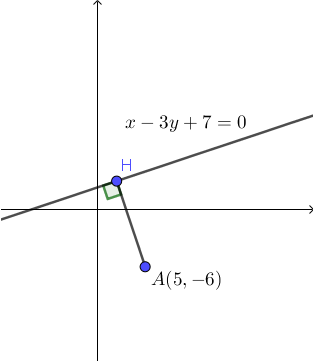
\includegraphics[width=0.4\textwidth]{distance_1}
\end{center}

\(A\)를 지나고 \(l\)에 수직한 직선의 방정식을 \(m:a'x+b'y+c'=0\)이라고 하자.
\(aa'+bb'=0\), 즉 \(a'-3b'=0\)을 만족시키게 하기 위해 \(a'=3\), \(b'=1\)로 잡으면
\[m:3x+y+c'=0\]
이 된다.
이 직선은 \(A(5,-6)\)을 지나므로 \(3\cdot5+(-6)+c'=0\)으로부터 \(c'=-9\)이다.
즉
\[m:3x+y-9=0\]
이다.
\(l\)과 \(m\)을 연립하기 위해 \(m\)의 식에 3을 곱해 \(l\)의 식과 더하면 \(10x-20=0\), \(x=2\)이다.
또 \(l\)의 식에 \(x=2\)를 대입하면 \(y=3\)이다.
즉 수선의 발 \(H\)의 좌표는 \(H=(2,3)\)이다.
따라서 수선 \(\ov AH\)의 길이는
\[d=\ov AH=\sqrt{(5-2)^2+(-6-3)^2}=3\sqrt{10}\]
이다.

%dist2
\prob{}\label{dist2}
점 \(A(1,2)\)과 직선 \(2x-y-5=0\) 사이의 거리 \(d\)를 구하여라.
\procedure{0.3}

\begin{mdframed}
%dist3
\theo{}\label{dist3}
점 \(A(x_1,y_1)\)과 직선 \(ax+by+c=0\)사이의 거리 \(d\)는
\[d=\frac{|ax_1+by_1+c|}{\sqrt{a^2+b^2}}\]
이다.
\end{mdframed}

%dist4
\exam{}\label{dist4}
예시 \ref{dist1})\을 정리 \ref{dist3})의 공식을 적용해 구하면
\[d=\frac{|5-3(-6)+7|}{\sqrt{1^2+(-3)^2}}=\frac{30}{\sqrt{10}}=3\sqrt{10}\]
이다.

%dist5
\prob{}\label{dist5}
문제 \ref{dist2})\를 정리 \ref{dist3})의 공식을 적용해 구하여라.

\clearpage
\bigskip\noindent\textsf{정리 \ref{dist3}의 증명)}\par
예시 \ref{dist1})에서 사용한 방법을 그대로 쓰면 증명할 수 있긴 하지만 점 \(H\)의 좌표를 구하는 부분과 그 이후가 아주 복잡하다.
따라서 \(H\)를 조금 다른 방법으로 구하여 증명하겠다.
\begin{center}
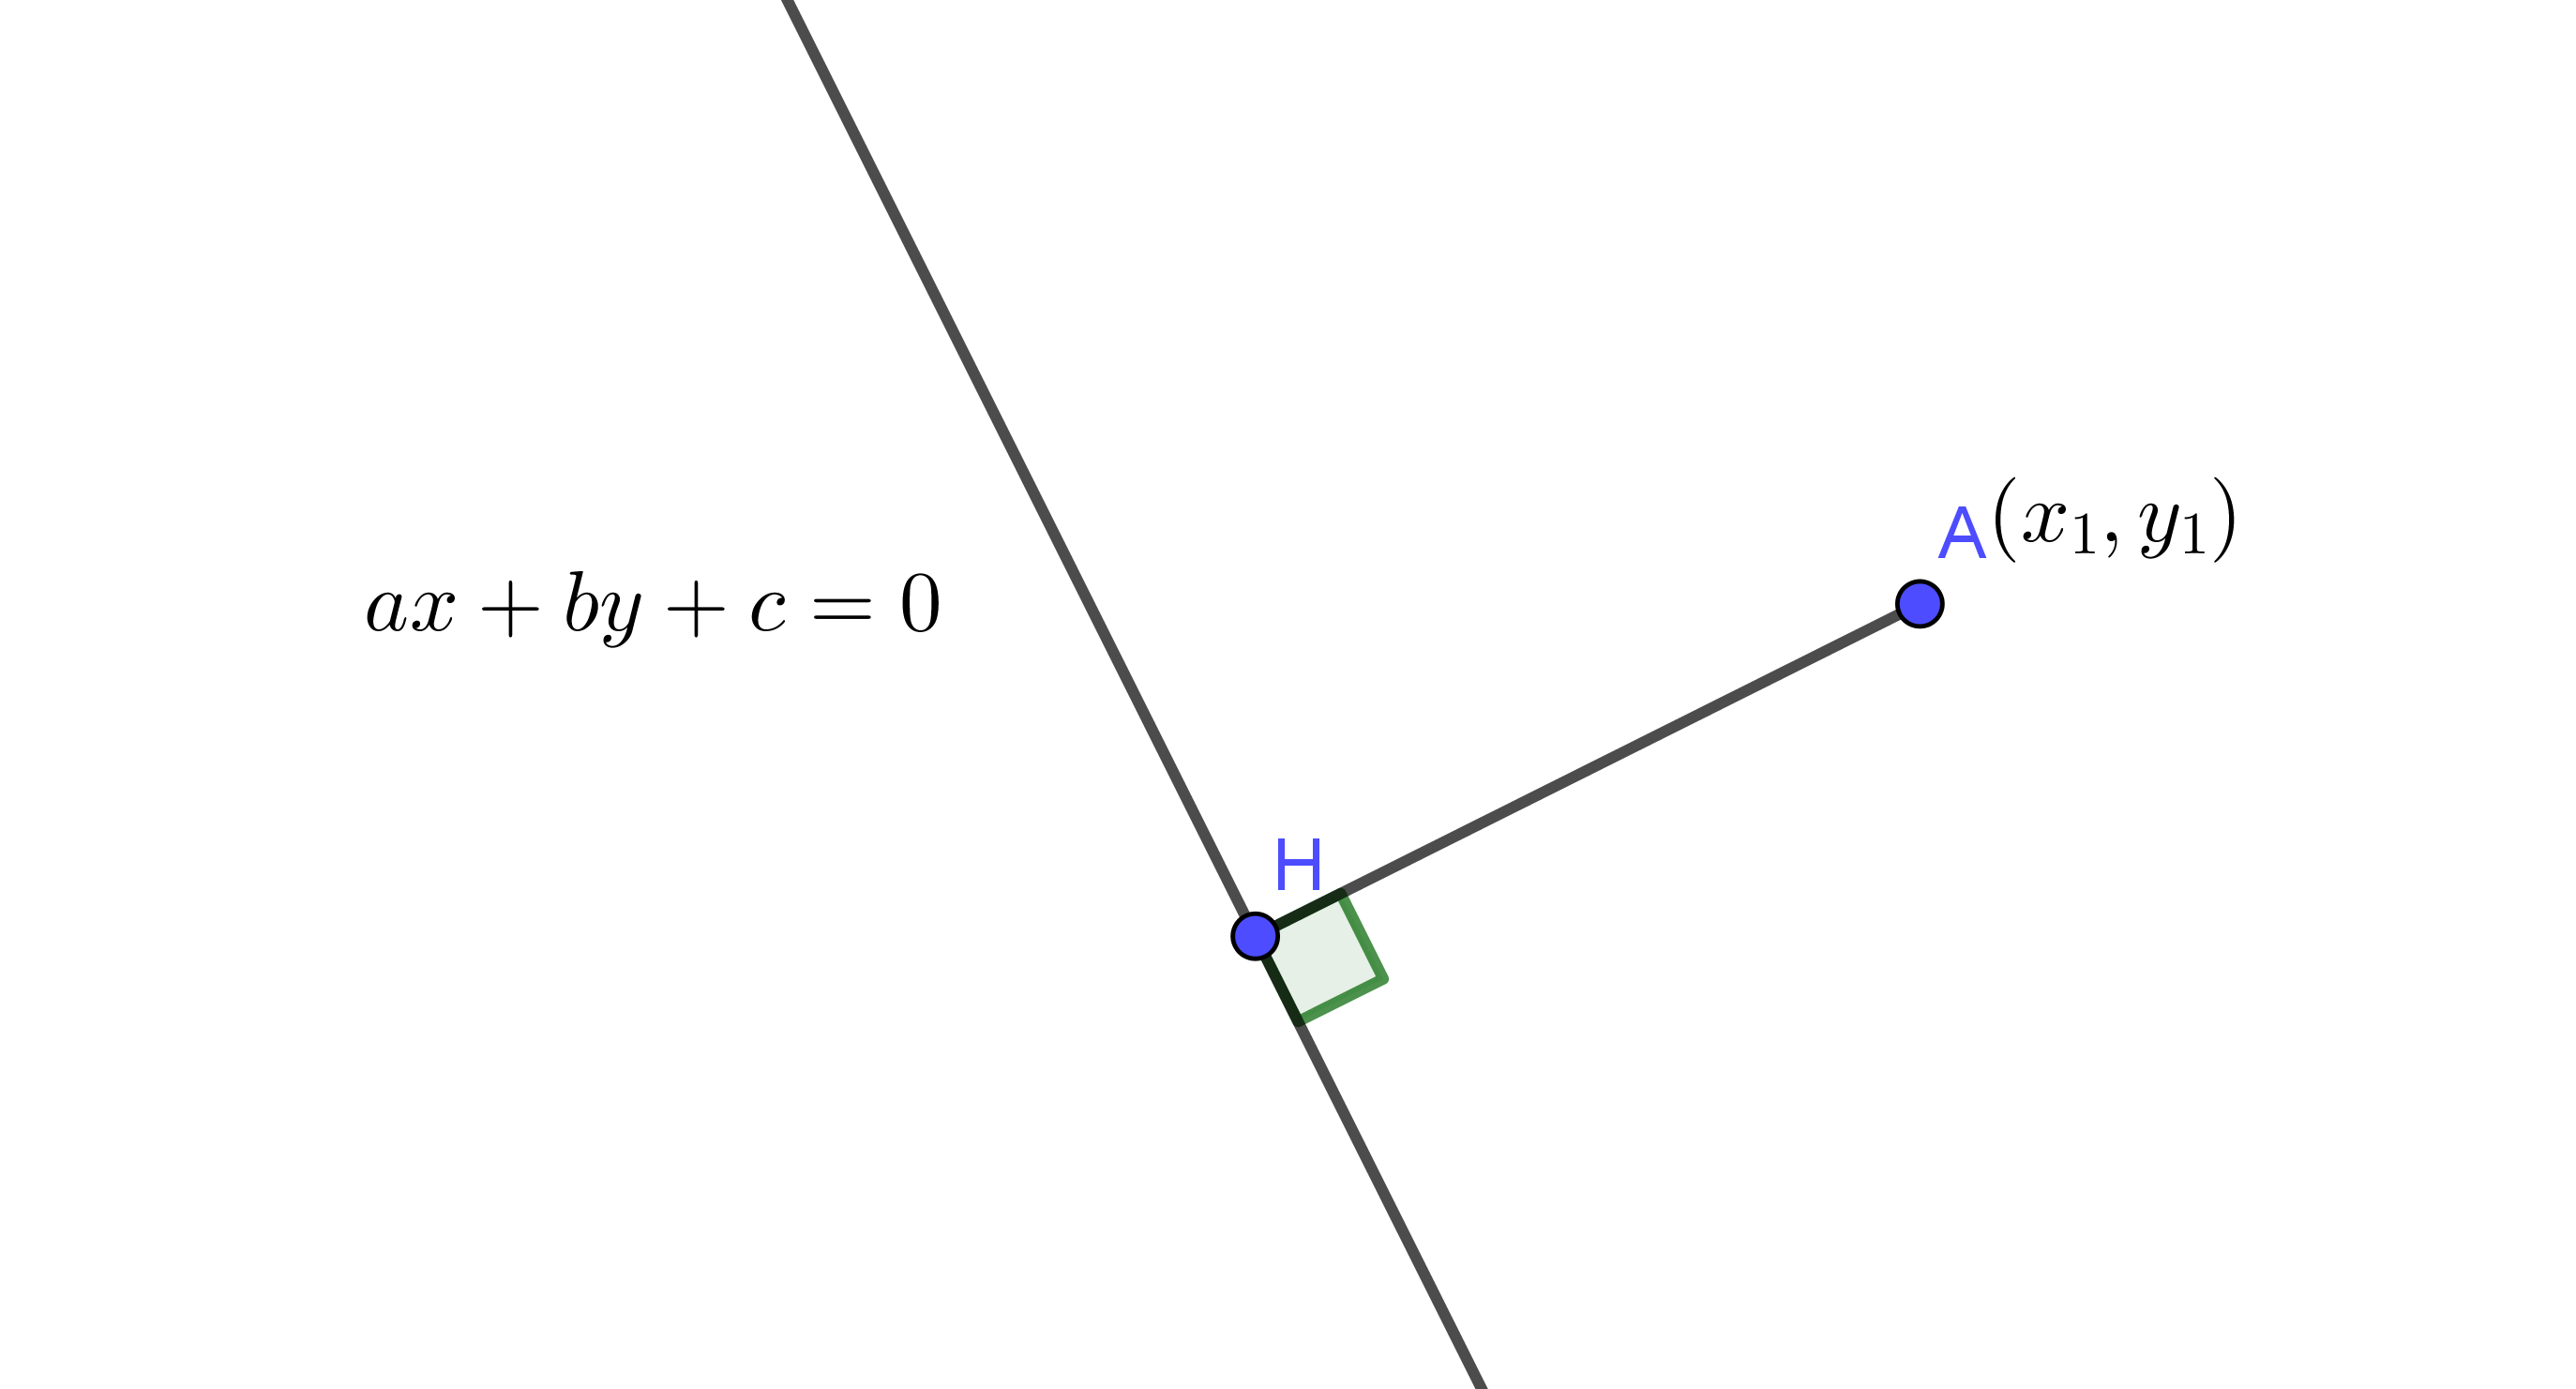
\includegraphics[width=0.7\textwidth]{distance_3}
\end{center}

\medskip
\(A(x_1,y_1)\)을 지나고 \(l:ax+by+c=0\)에 수직한 직선의 방정식을
\[m:a'x+b'y+c'=0\]
이라고 하자.
\(aa'+bb'=0\)을 만족하도록 \(a'\)과 \(b'\)을 \(a'=b\), \(b'=-a\)로 잡으면
\[m:bx-ay+c'=0\]
이다.
이 직선은 \(A(x_1,y_1)\)을 지나므로 \(bx_1-ay_1+c'=0\)으로부터 \(c'=-bx_1+ay_1\)이다.
즉,
\[m:bx-ay-bx_1+ay_1=0\]
이 된다.
이것을 정리하면
\[m:b(x-x_1)=a(y-y_1)\]
으로 쓸 수도 있다.

\medskip
\(A\)에서 \(l\)에 내린 수선의 발을 \(H\)라고 하자.
\(H\)의 \(x\)좌표를 \(x_1+at\)로 잡으면 \(H\)는 직선 \(m\) 위의 점이므로
\begin{gather*}
b\left((x_1+at)-x_1\right)=a(y-y_1)\\
abt=a(y-y_1)\\
bt=y-y_1
\end{gather*}
가 성립해야 한다. 즉
\[y=y_1+bt\]
이다.
따라서
\[H=(x_1+at,y_1+bt)\]
로 놓을 수 있다.

\medskip
\(H\)는 직선 \(l\) 위의 점이기도 하므로
\begin{gather*}
a(x_1+at)+b(y_1+bt)+c=0\\
(a^2+b^2)t+(ax_1+by_1+c)=0\\
t=-\frac{ax_1+by_1+c}{a^2+b^2}
\end{gather*}
이다.

\medskip
이제 \(d\)를 구하면
\begin{align*}
d
&=\ov AH\\
&=\sqrt{\left(x_1-(x_1+at)\right)^2+\left(y_1-(y_1+bt)\right)^2}\\
&=\sqrt{(a^2+b^2)t^2}\\
&=|t|\sqrt{a^2+b^2}\\
&=\frac{|ax_1+by_1+c|}{a^2+b^2}\sqrt{a^2+b^2}\\
&=\frac{|ax_1+by_1+c|}{\sqrt{a^2+b^2}}
\end{align*}
이다.
\qed

%%
\section*{답}
\addcontentsline{toc}{chapter}{\protect\numberline{*}답}
%
\an{line2}
\(2\), \(1\), \(2\), \(1\), \(-\frac13\), \(-\frac13\), \(-\frac13\), \(3\), \(3\), \(3\)

%
\an{line5}
\(y=\sqrt3x+1\)

%
\an{lline3}
\footnotesize
\begin{minipage}{0.45\textwidth}
\par\medskip
\begin{minipage}{0.45\textwidth}\centering
\(y=x+2\)
\par\bigskip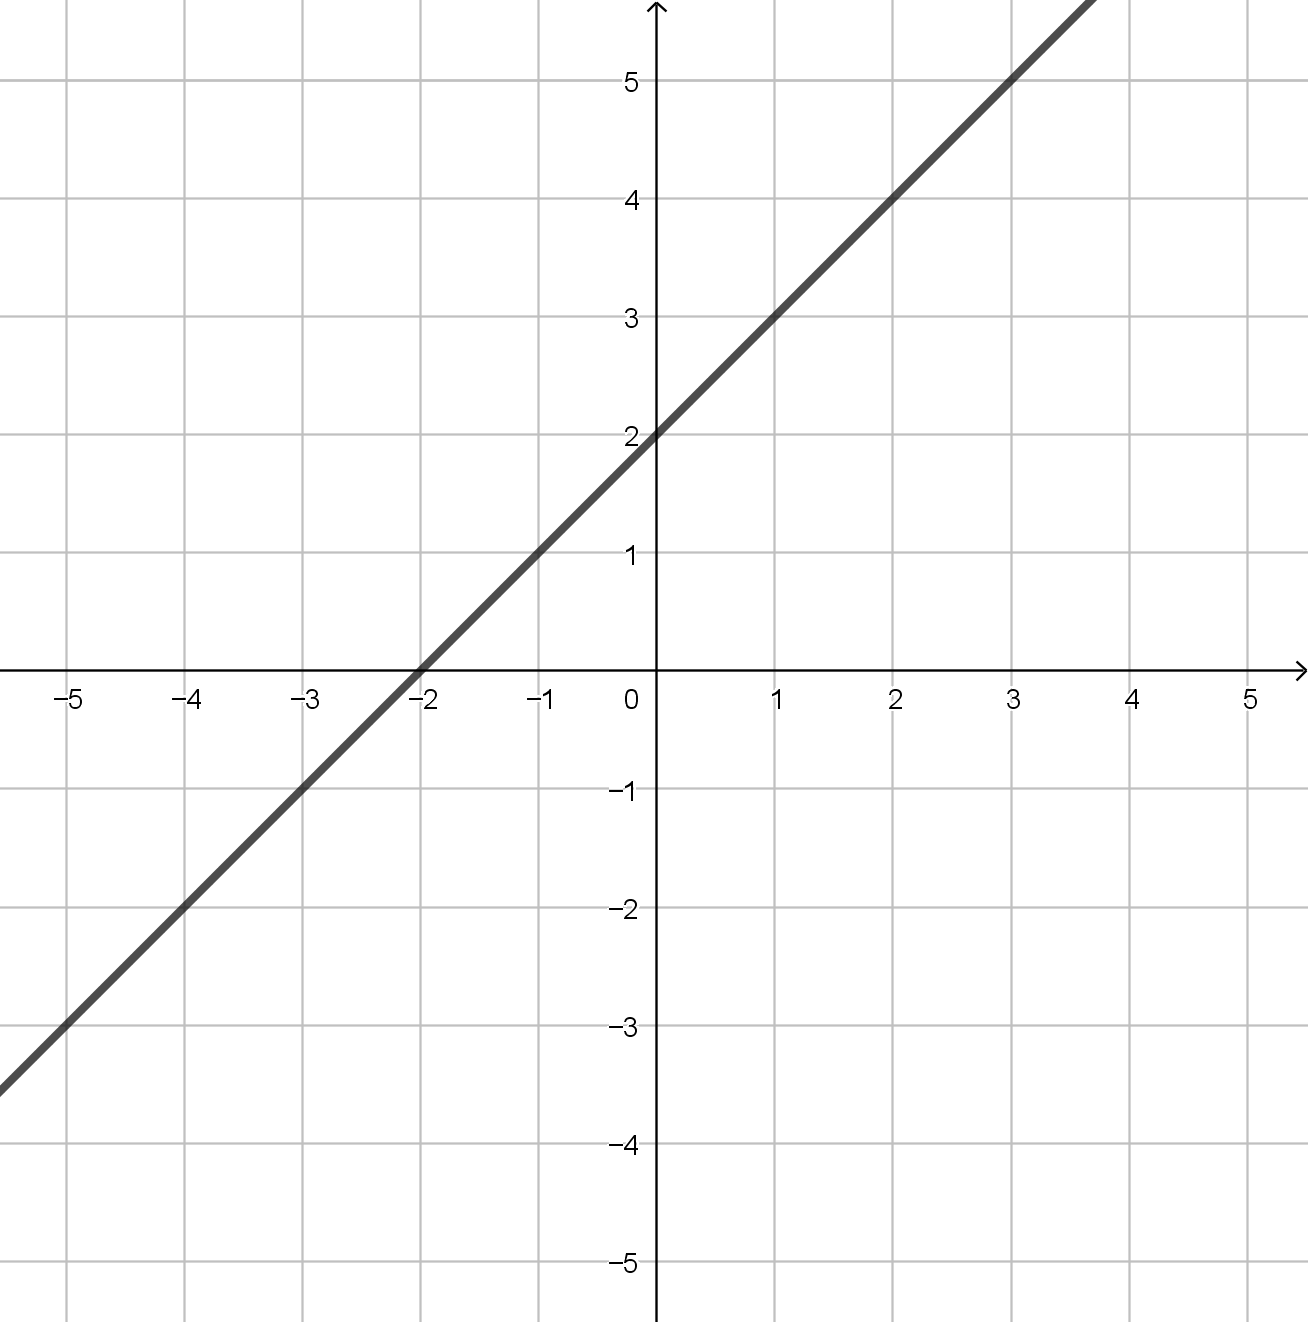
\includegraphics[width=0.9\textwidth]{L01}
\end{minipage}
\begin{minipage}{0.45\textwidth}\centering
\(y=3x-3\)
\par\bigskip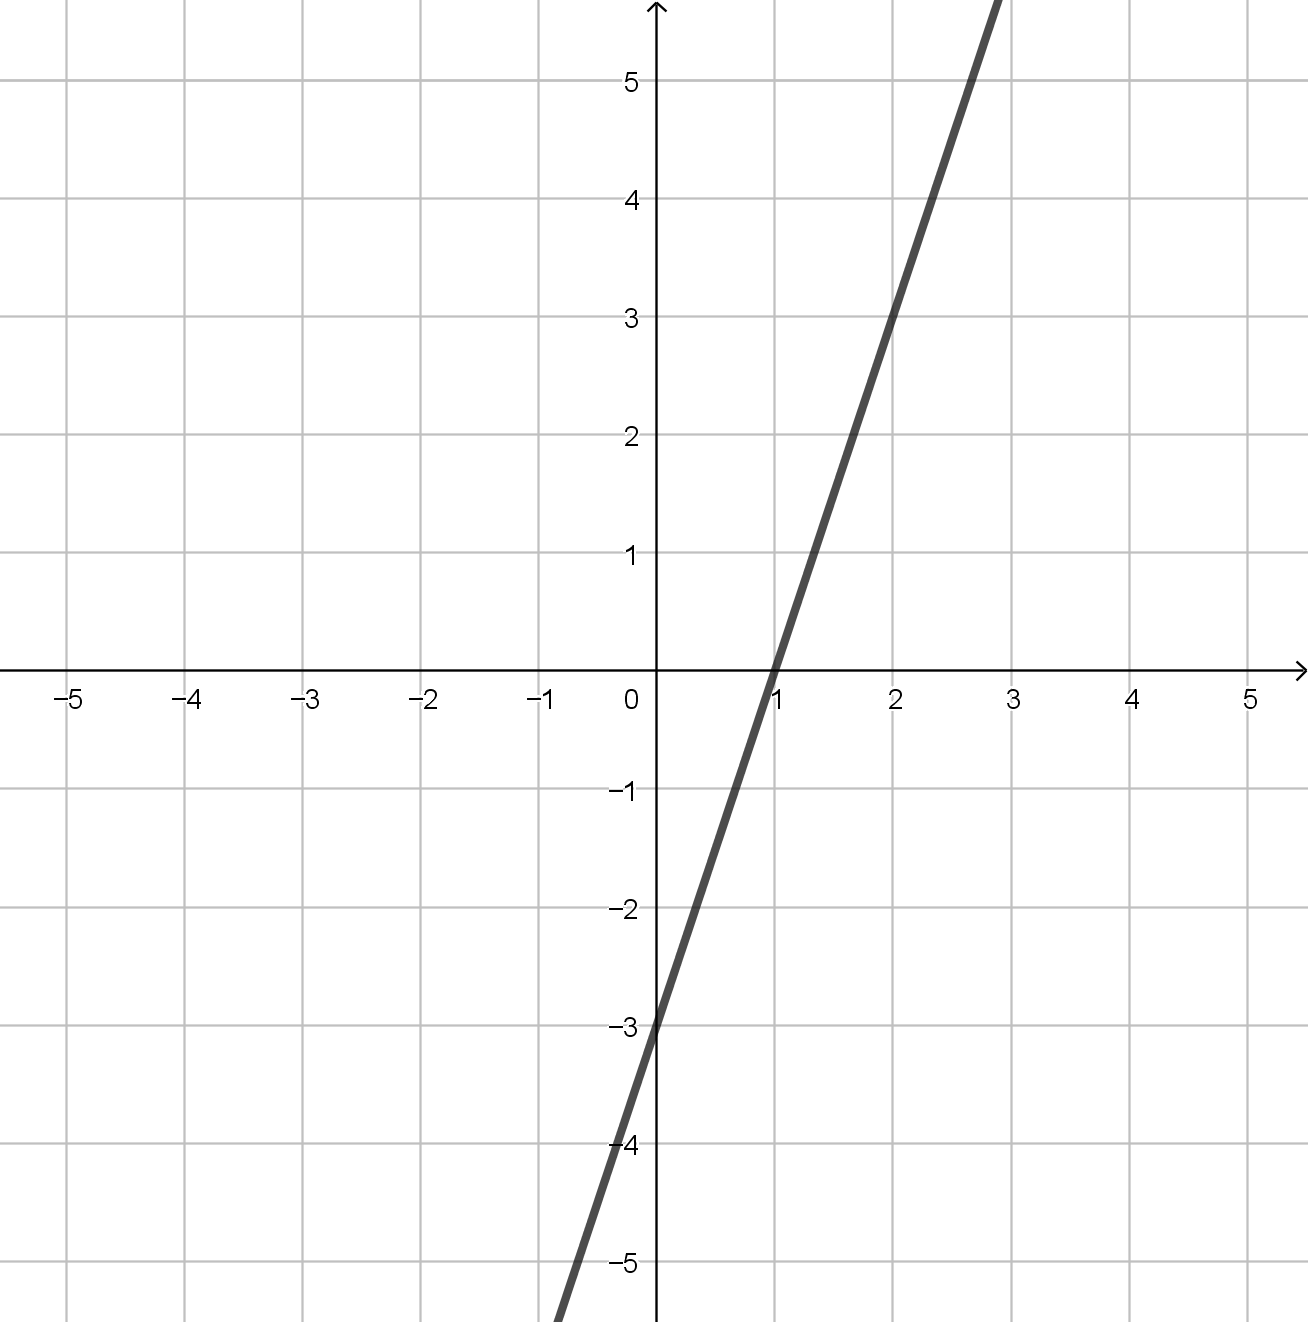
\includegraphics[width=0.9\textwidth]{L02}
\end{minipage}\bigskip\bigskip\par
\begin{minipage}{0.45\textwidth}\centering
\(y=-3x+5\)
\par\bigskip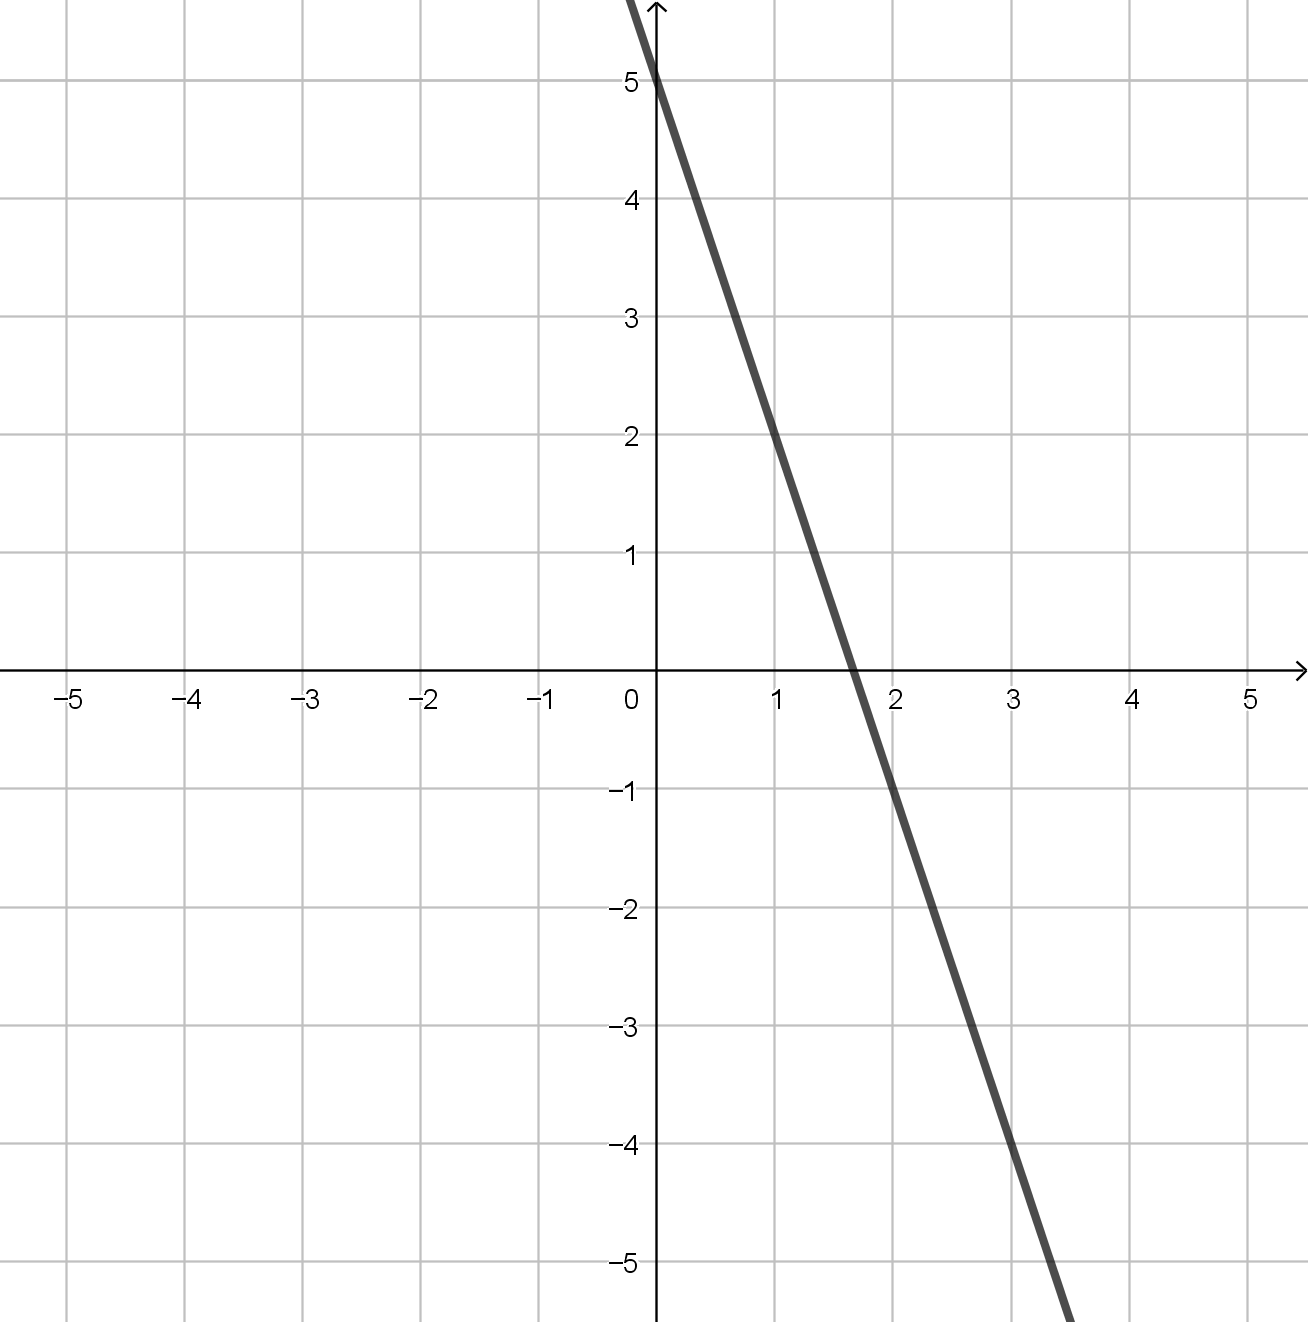
\includegraphics[width=0.9\textwidth]{L03}
\end{minipage}
\begin{minipage}{0.45\textwidth}\centering
\(y=-2x\)
\par\bigskip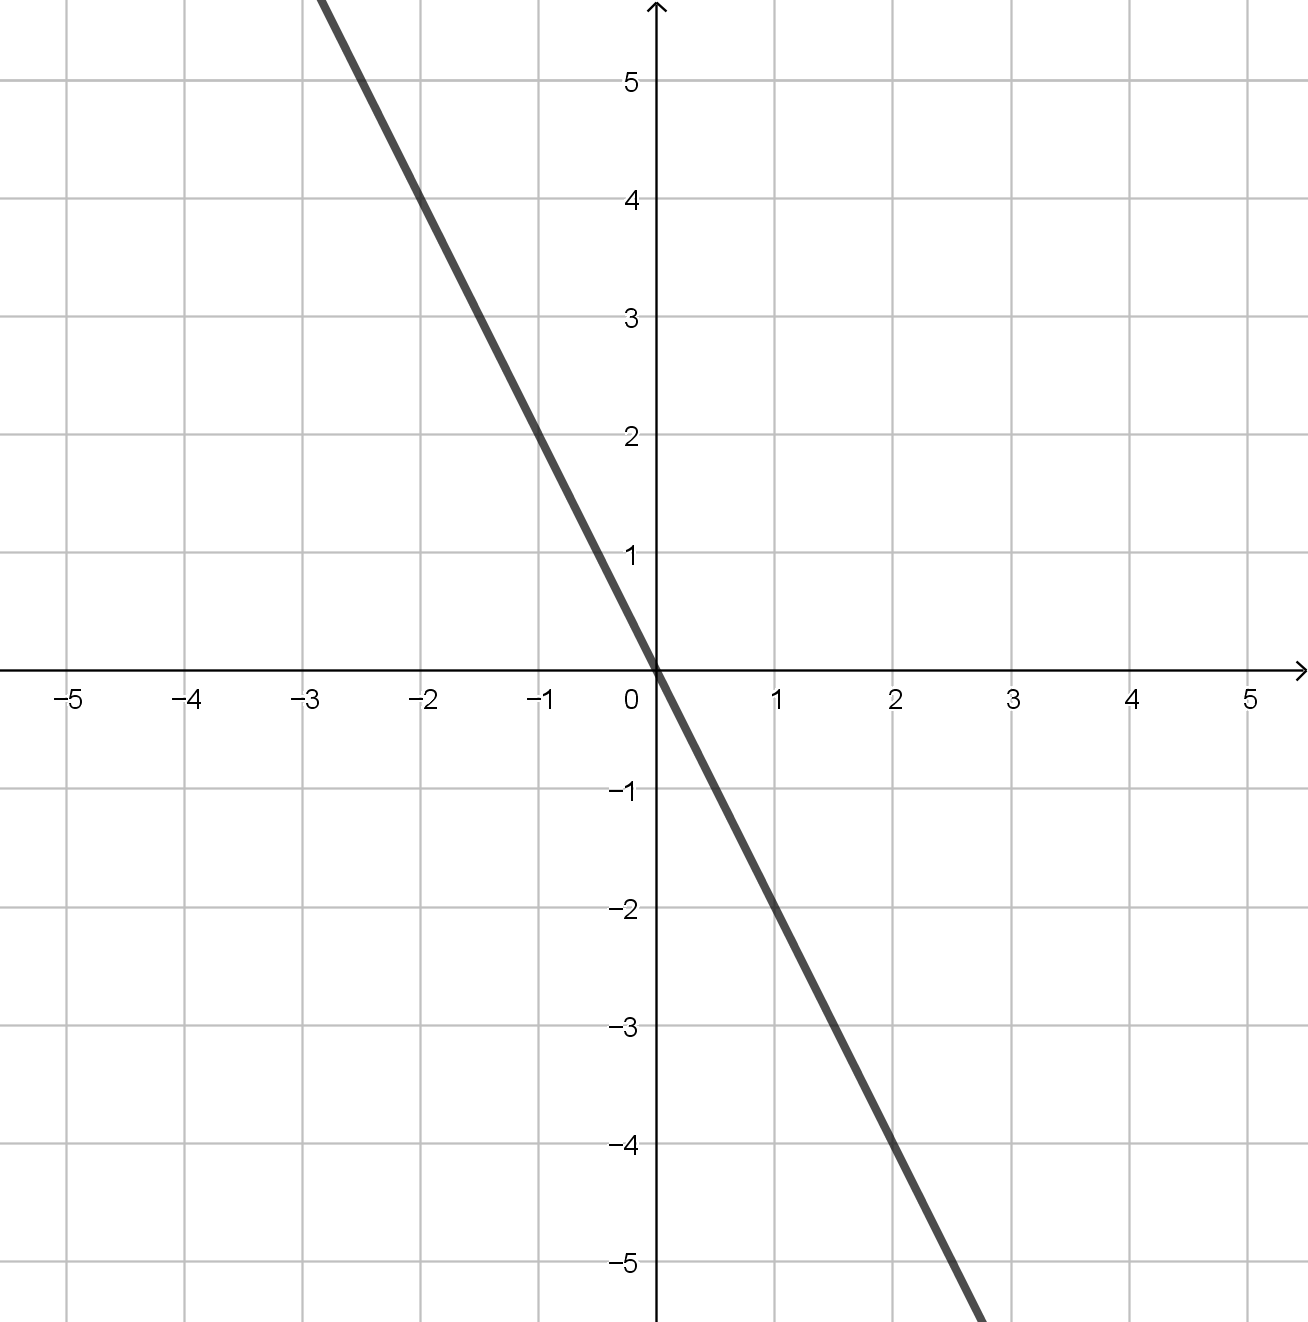
\includegraphics[width=0.9\textwidth]{L04}
\end{minipage}\bigskip\bigskip\par
\begin{minipage}{0.45\textwidth}\centering
\(y=\frac12x-2\)
\par\bigskip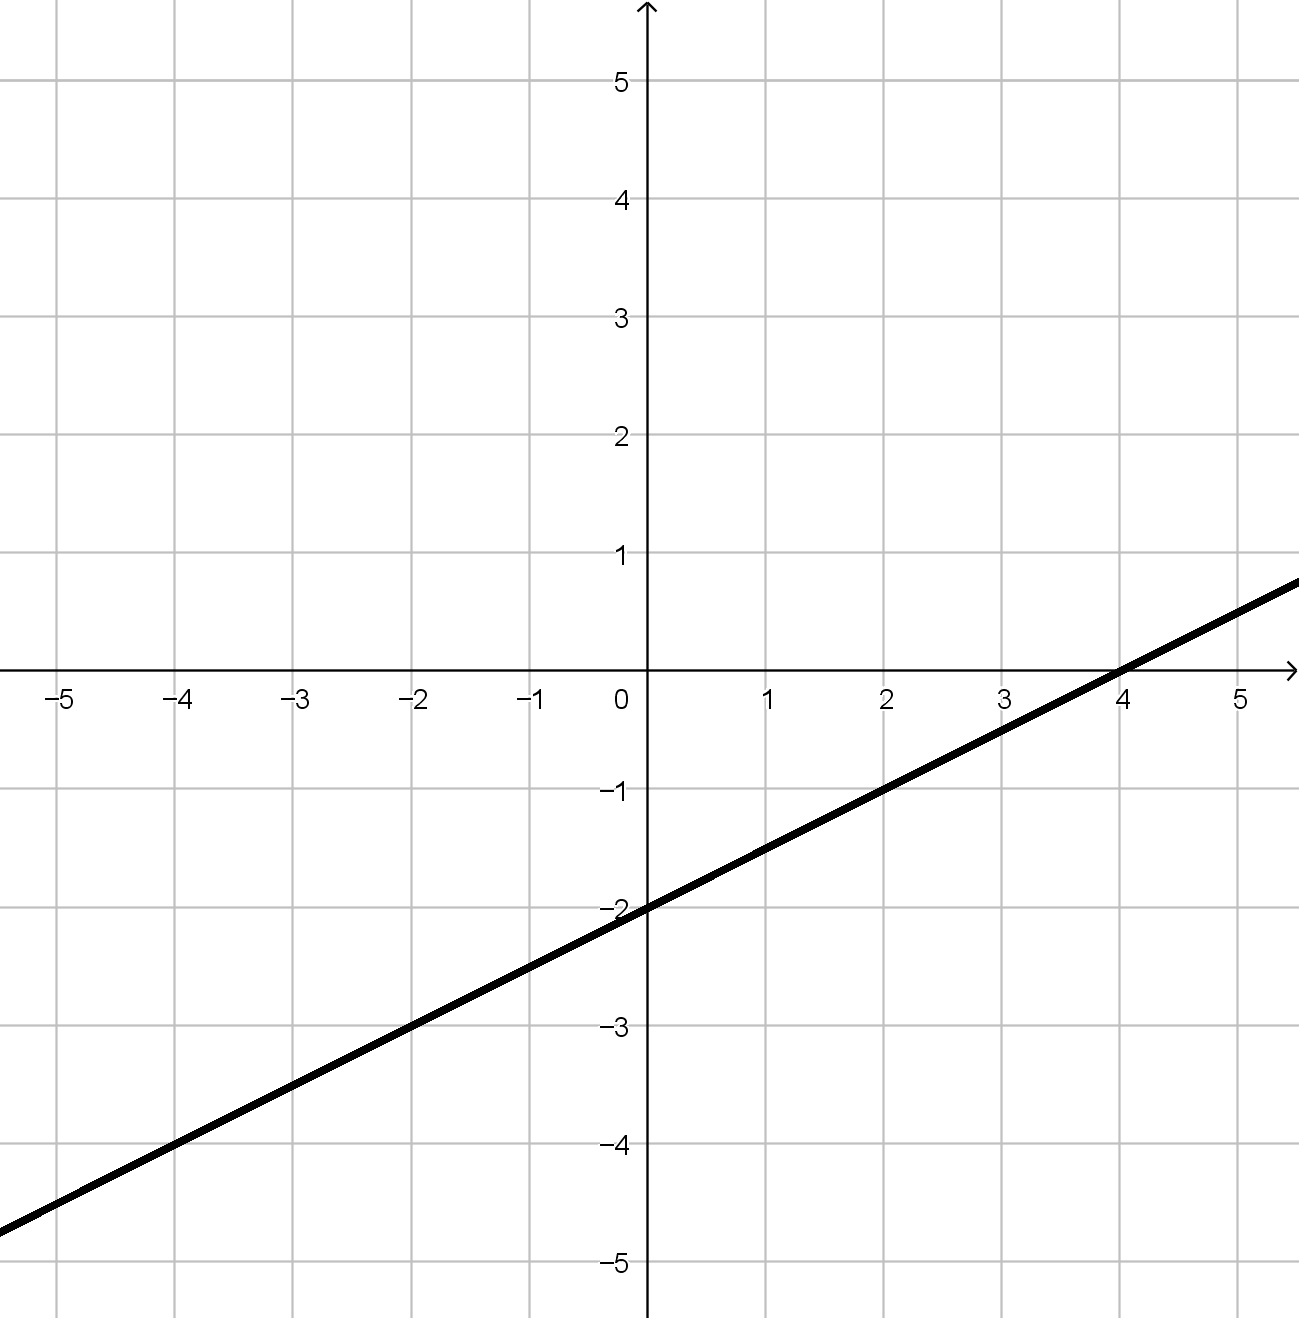
\includegraphics[width=0.9\textwidth]{L05}
\end{minipage}
\begin{minipage}{0.45\textwidth}\centering
\(y=-\frac23x+1\)
\par\bigskip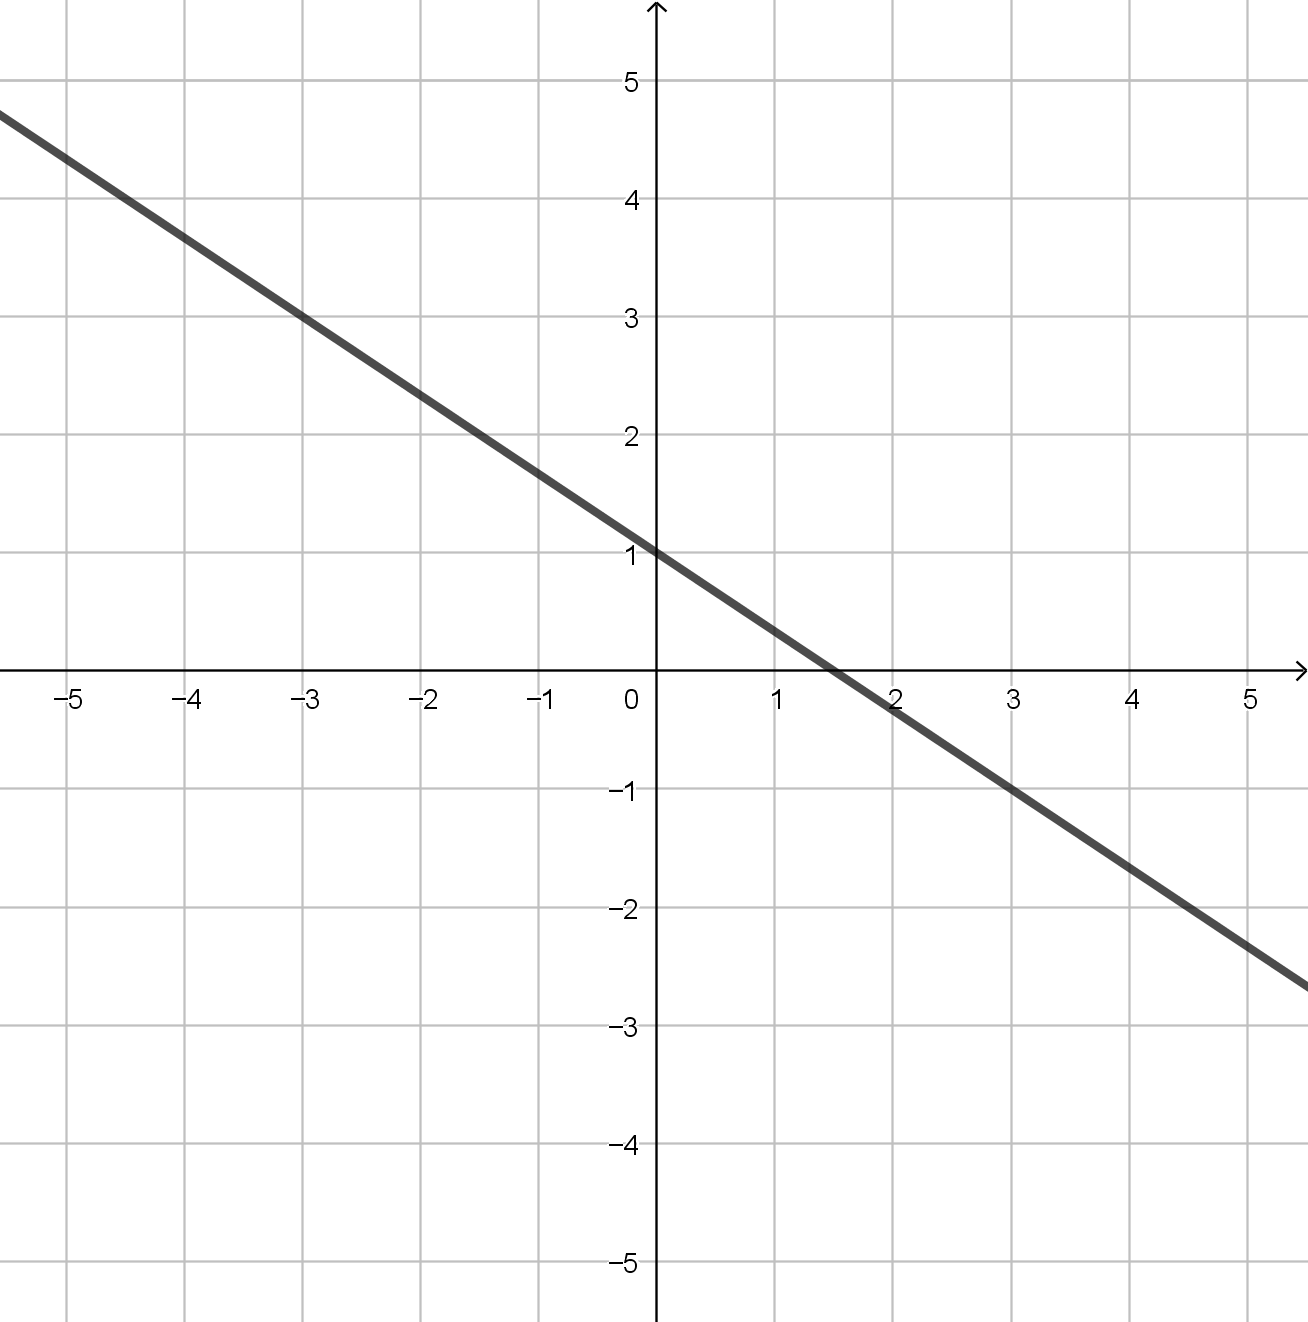
\includegraphics[width=0.9\textwidth]{L06}
\end{minipage}\bigskip\bigskip\par
\end{minipage}
%
\begin{minipage}{0.45\textwidth}
\clearpage
\begin{minipage}{0.45\textwidth}\centering
\(2x+y-1=0\)
\par\bigskip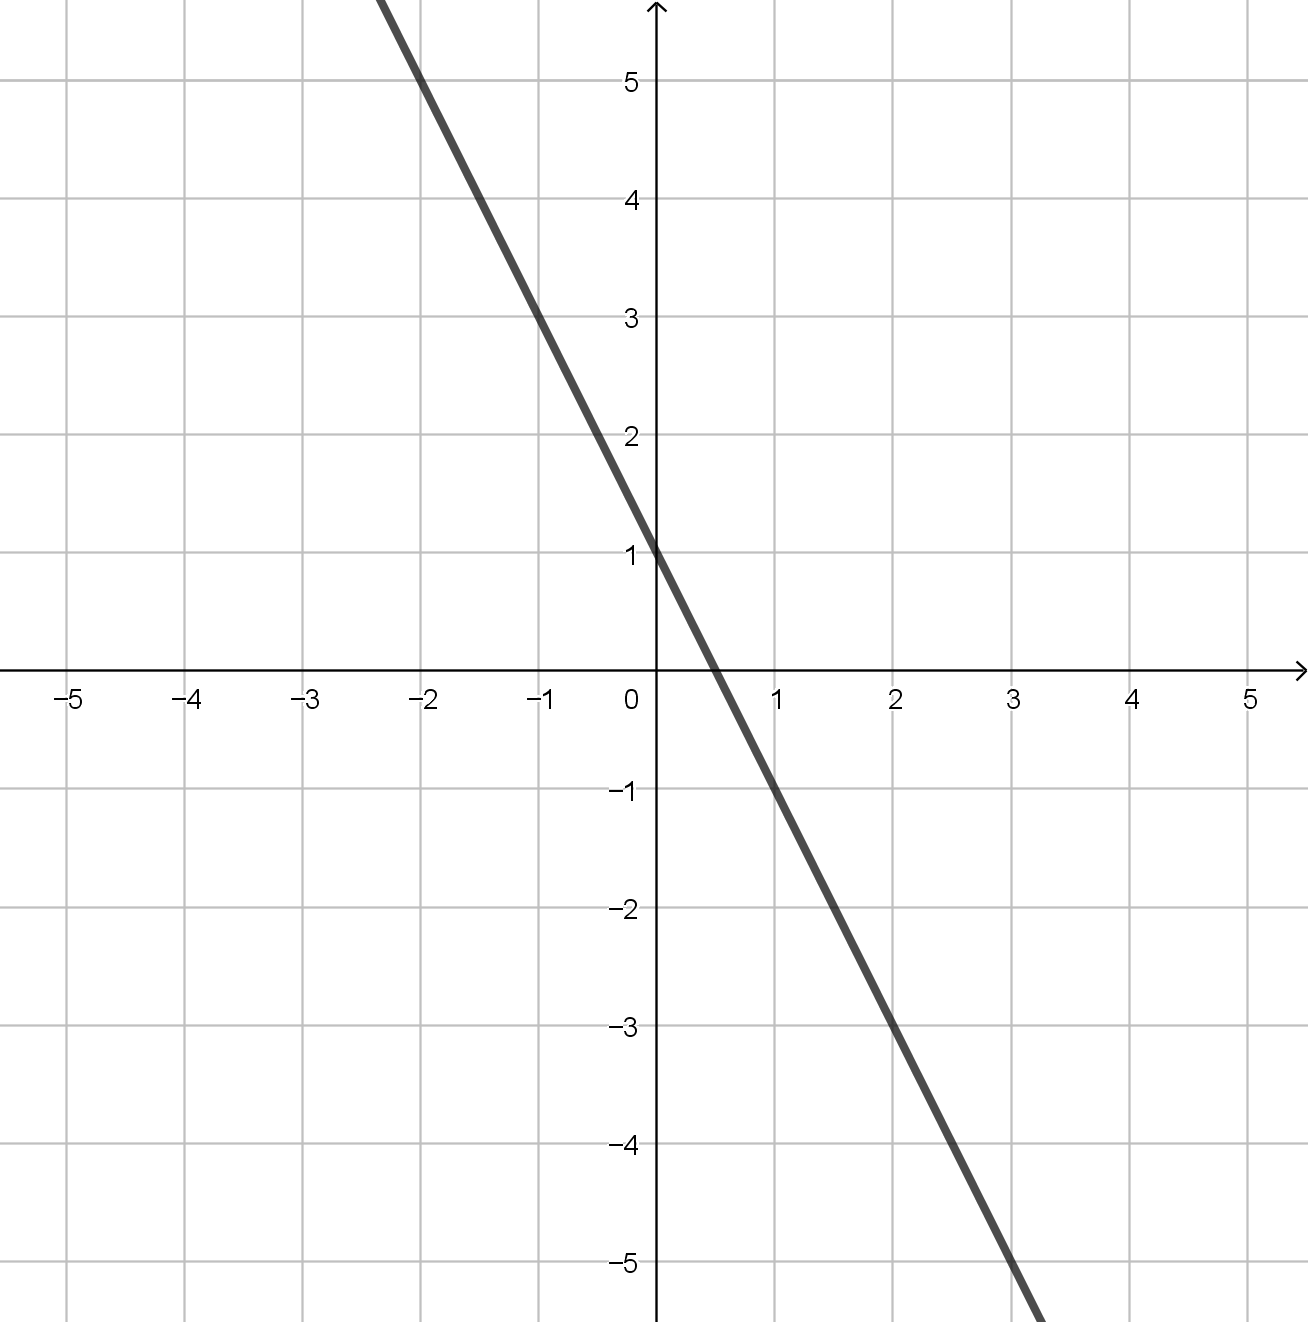
\includegraphics[width=0.9\textwidth]{L07}
\end{minipage}
\begin{minipage}{0.45\textwidth}\centering
\(2x+3y+6=0\)
\par\bigskip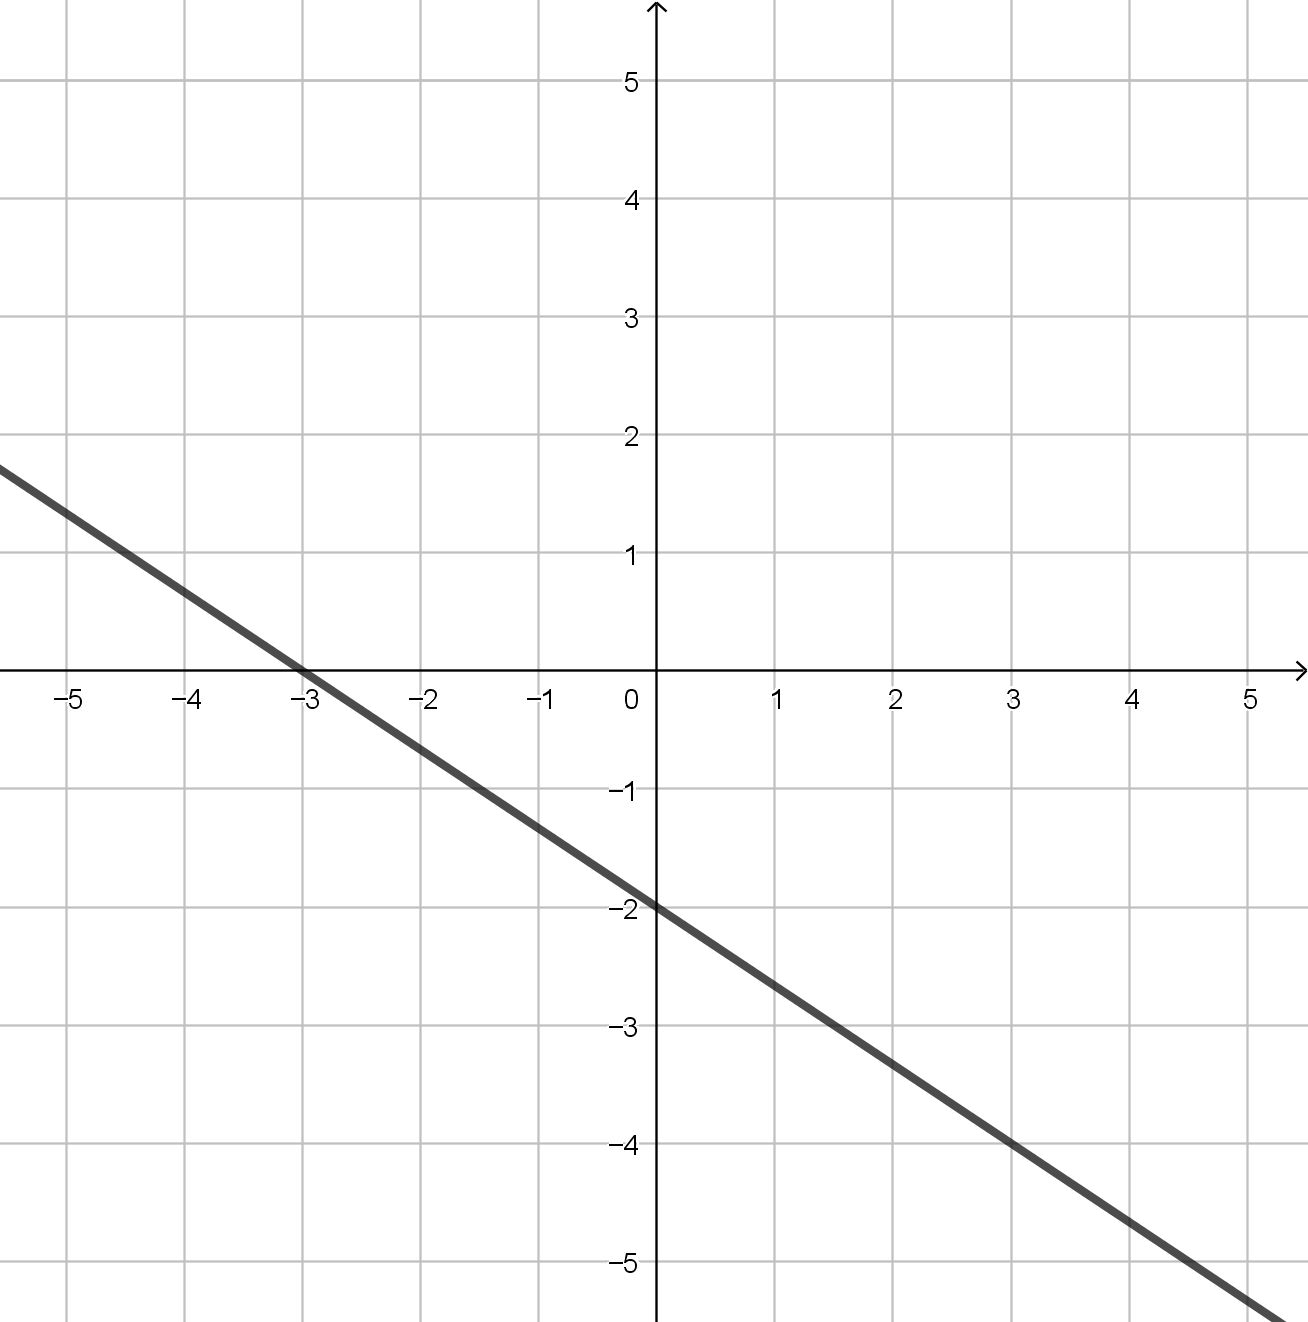
\includegraphics[width=0.9\textwidth]{L08}
\end{minipage}\bigskip\bigskip\par
\begin{minipage}{0.45\textwidth}\centering
\(x+y=2\)
\par\bigskip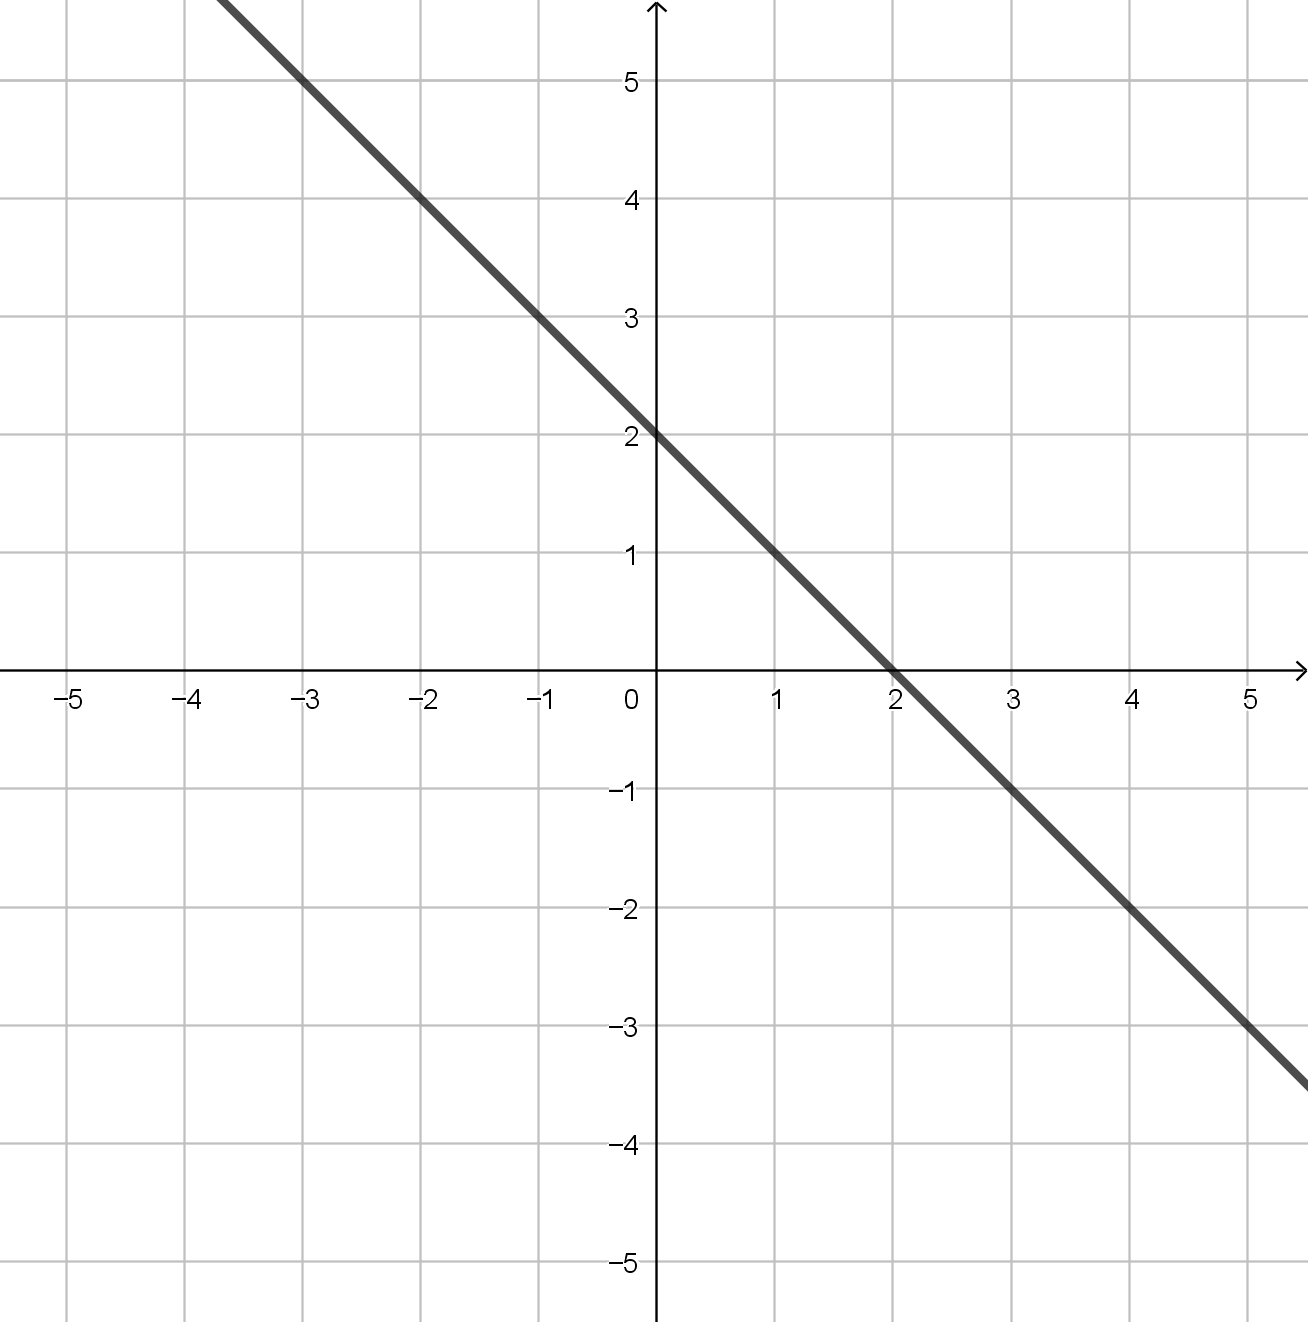
\includegraphics[width=0.9\textwidth]{L09}
\end{minipage}
\begin{minipage}{0.45\textwidth}\centering
\(y=-1\)
\par\bigskip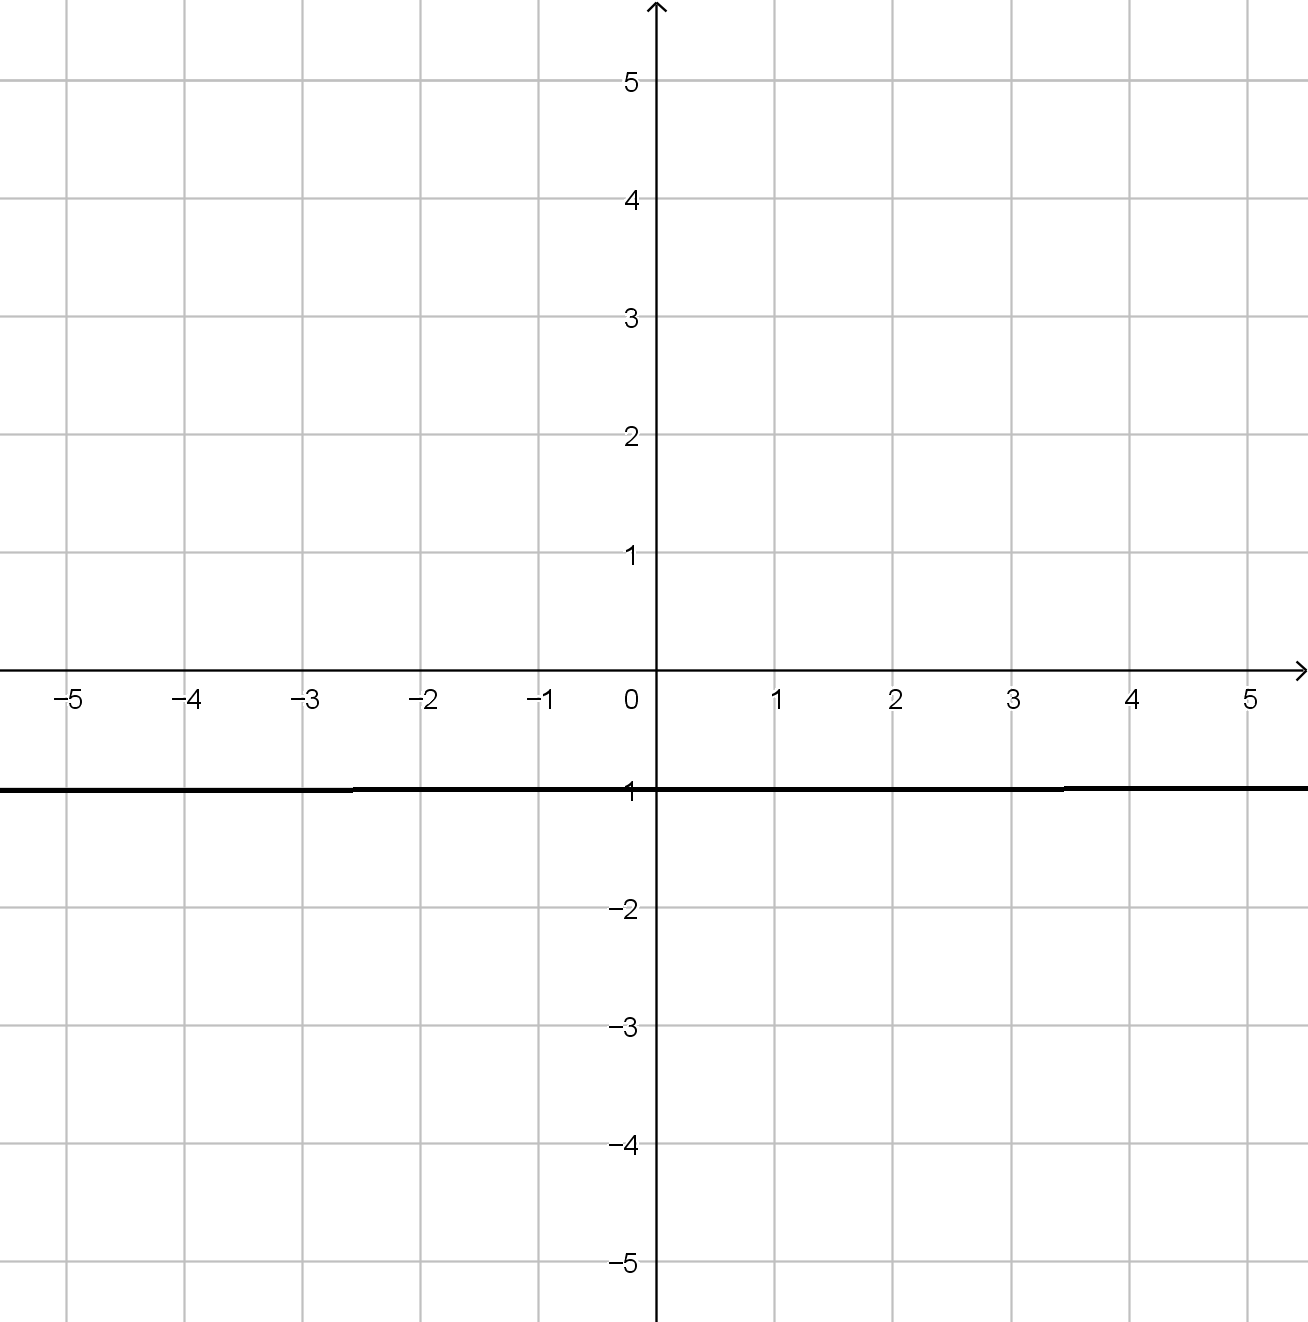
\includegraphics[width=0.9\textwidth]{L10}
\end{minipage}\bigskip\bigskip\par
\begin{minipage}{0.45\textwidth}\centering
\(x=-1\)
\par\bigskip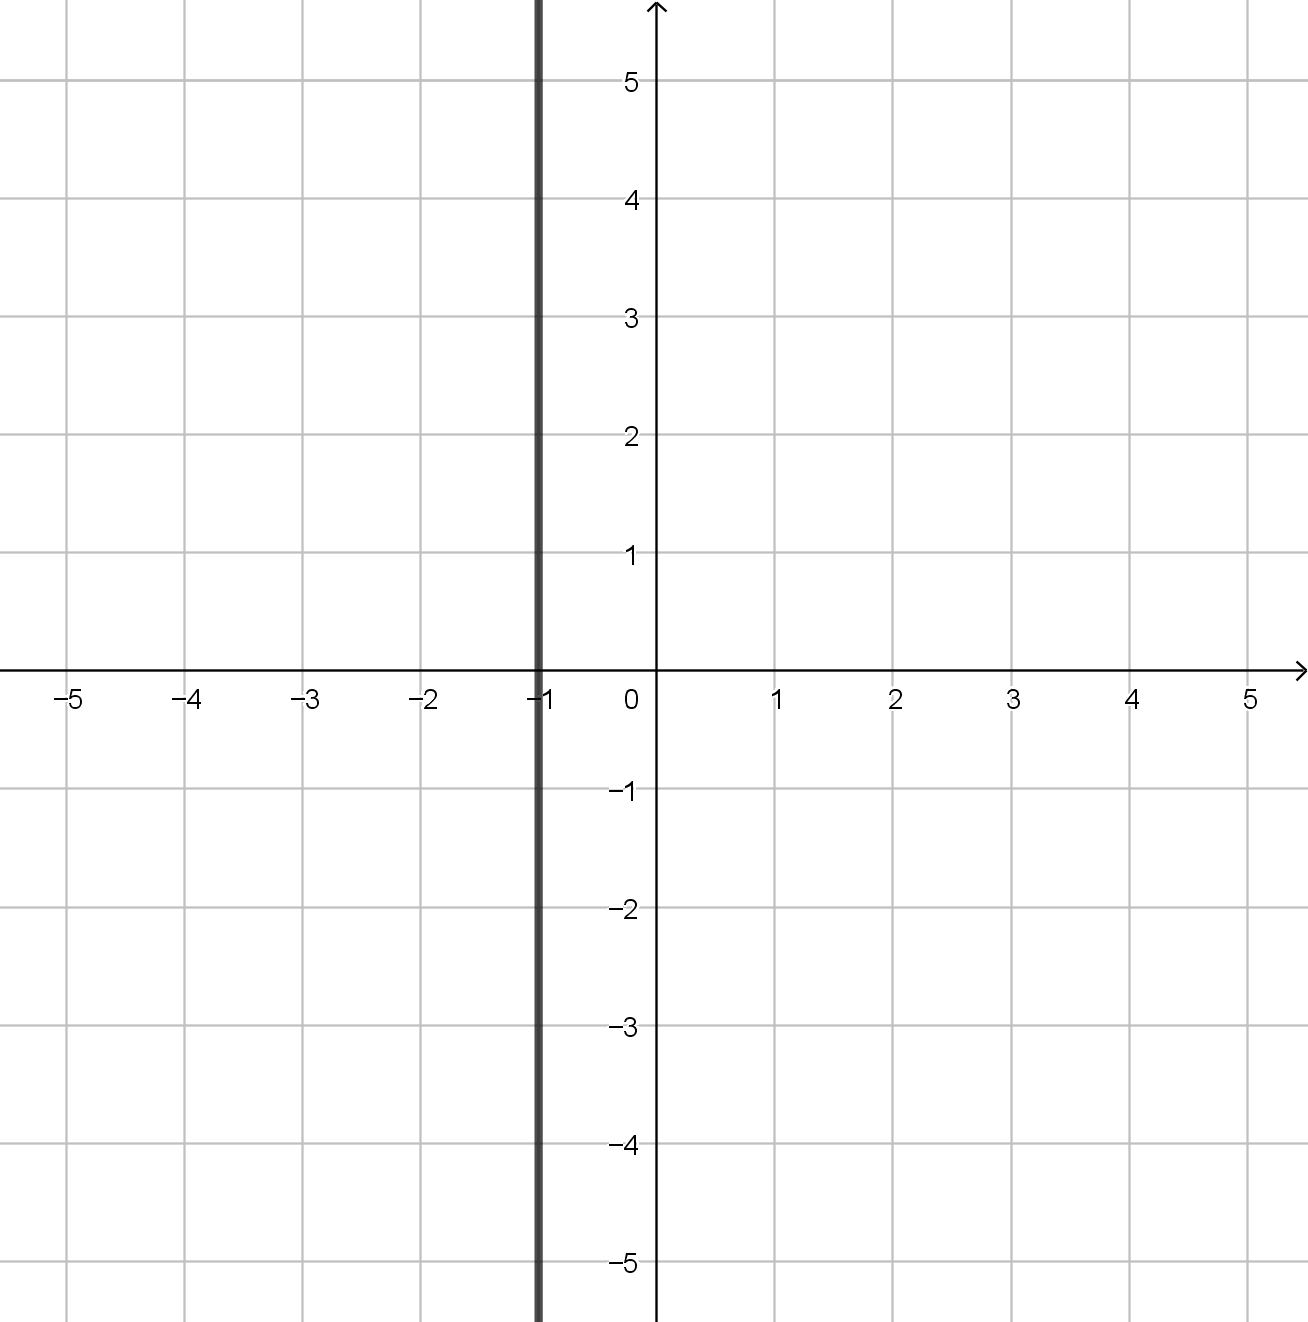
\includegraphics[width=0.9\textwidth]{L11}
\end{minipage}
\begin{minipage}{0.45\textwidth}\centering
\(x=0\)
\par\bigskip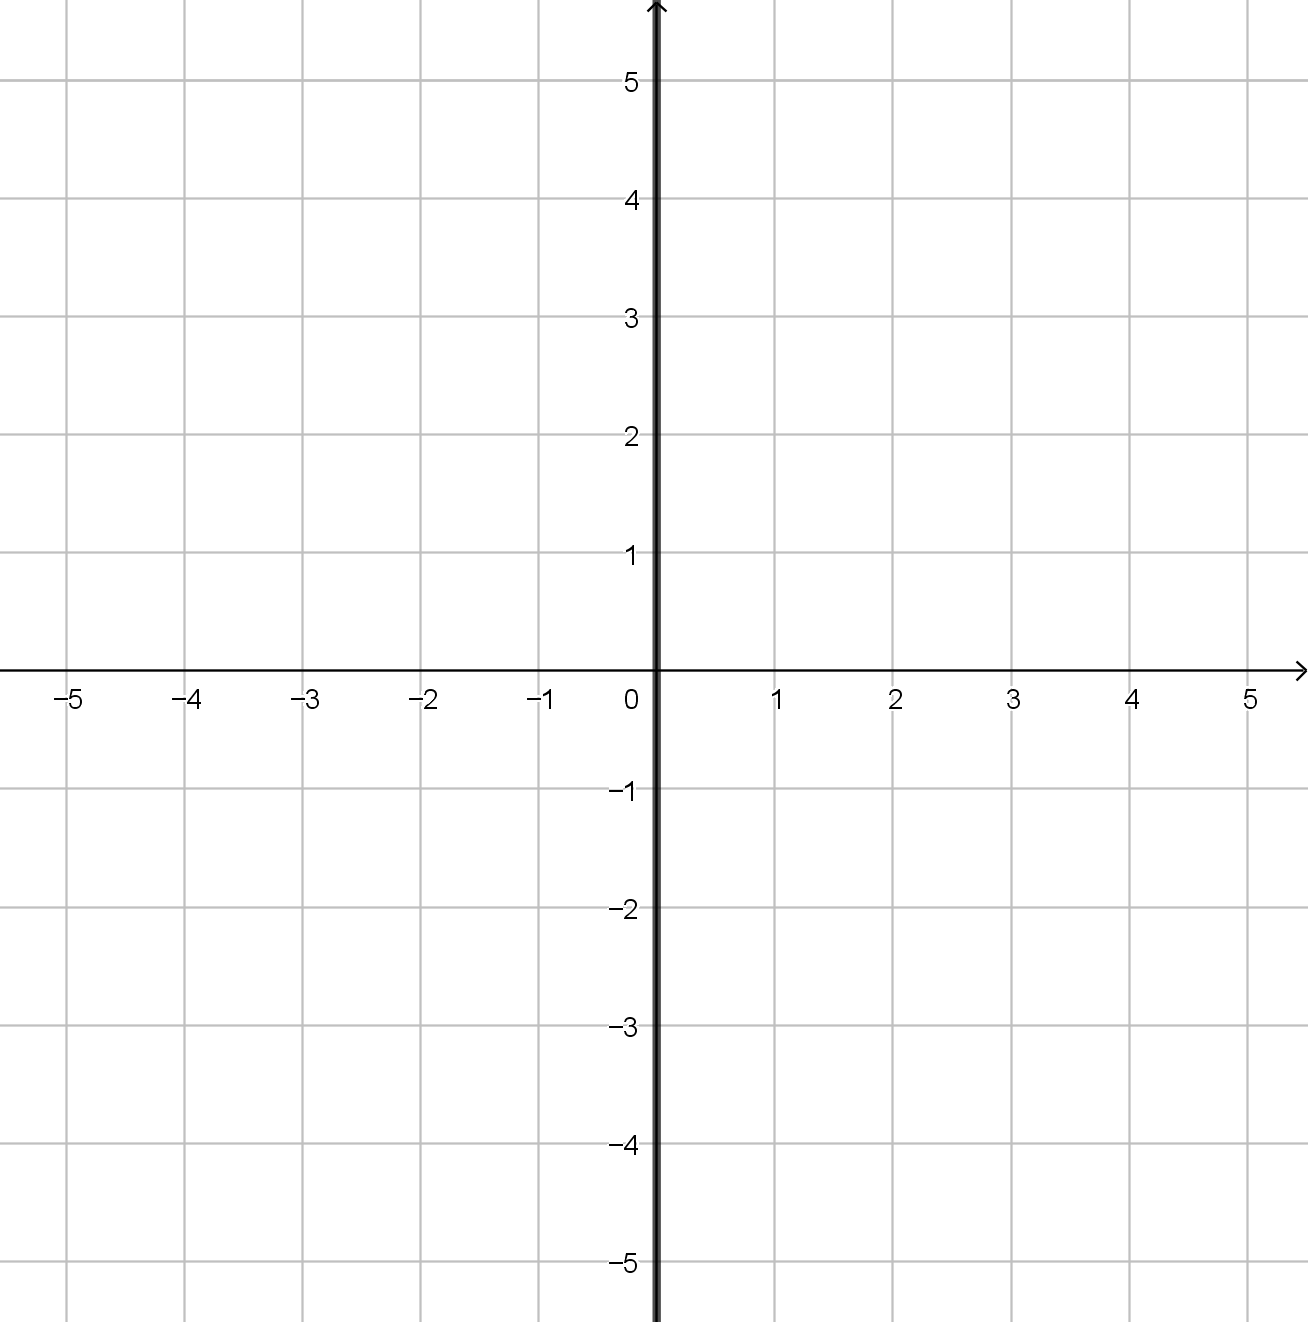
\includegraphics[width=0.9\textwidth]{L12}
\end{minipage}\bigskip\bigskip\par
\end{minipage}
\normalsize

\begin{minipage}[t]{.49\textwidth}
%
\an{two3}
\(0\)

%
\an{two4}
\(a\neq2\)

%
\an{two5}
\(3\)

%
\an{two6}
\(-3\)

%
\an{two7}
\(-1\)

%
\an{two10}
\(-\frac23\)

%
\an{two11}
\(-3\)

%
\an{two12}
\(-1\)

%
\an{two13}
\(8\)

\end{minipage}
\begin{minipage}[t]{.49\textwidth}

%
\an{three2}
\(y=\frac12x+4\)

%
\an{three5}
생략

%
\an{three8}
\(y=5x-16\)

%
\an{three11}
\(x+6y-3=0\)

%
\an{inter4}
\(2x-y-1=0\)

%
\an{inter5}
\(y=-3x+6\)

%
\an{dist2}
\(\sqrt5\)

%
\an{dist4}
생략
\end{minipage}

%%
\section*{요약}
\addcontentsline{toc}{chapter}{\protect\numberline{*}요약}
\begin{enumerate}[label=\emph{\arabic*.},itemsep=10pt]
\item
\(y=mx+n\)
\begin{itemize}
\item
\(m=기울기=\frac{\Delta y}{\Delta x}=\tan\alpha\)
\item
\(n=y절편\)
\end{itemize}
\item
\(ax+by+c=0\)
\begin{itemize}
\item
\(y=-\frac abx-\frac cb\)
\item
\(a=0\)이면 \(x\)축에 평행한 그래프
\item
\(b=0\)이면 \(y\)축에 평행한 그래프
\end{itemize}
\item
두 직선의 위치관계\\[10pt]
\begin{tabu}to.8\textwidth{X[2,c]|X[2,c]|X[2,c]}
\toprule
일치한다	&평행하다	&한 점에서 만난다\\
\hline
 \raisebox{-.5\height}{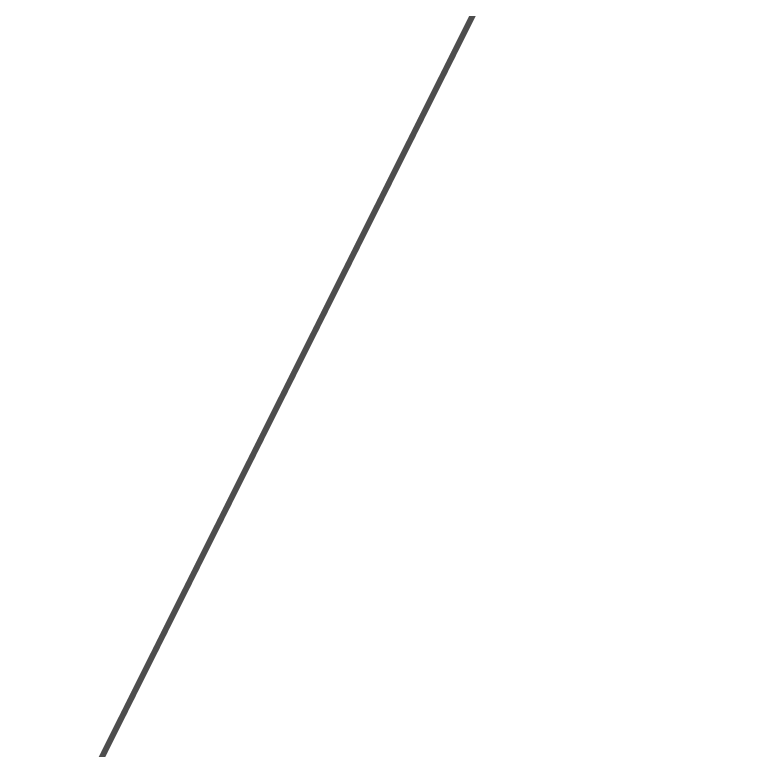
\includegraphics[width=0.12\textwidth]{twolines_1}}
&\raisebox{-.5\height}{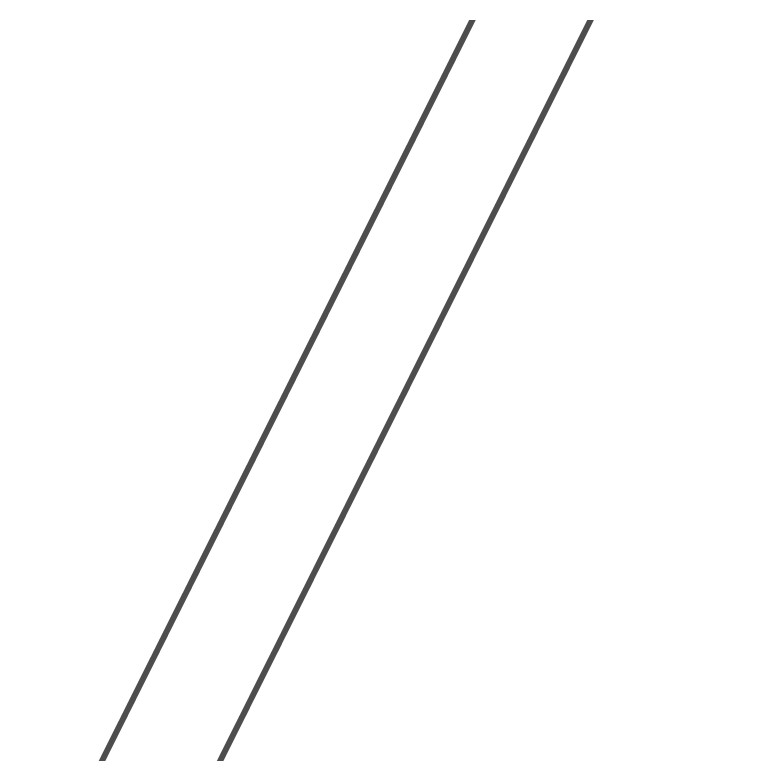
\includegraphics[width=0.12\textwidth]{twolines_2}}
&\raisebox{-.5\height}{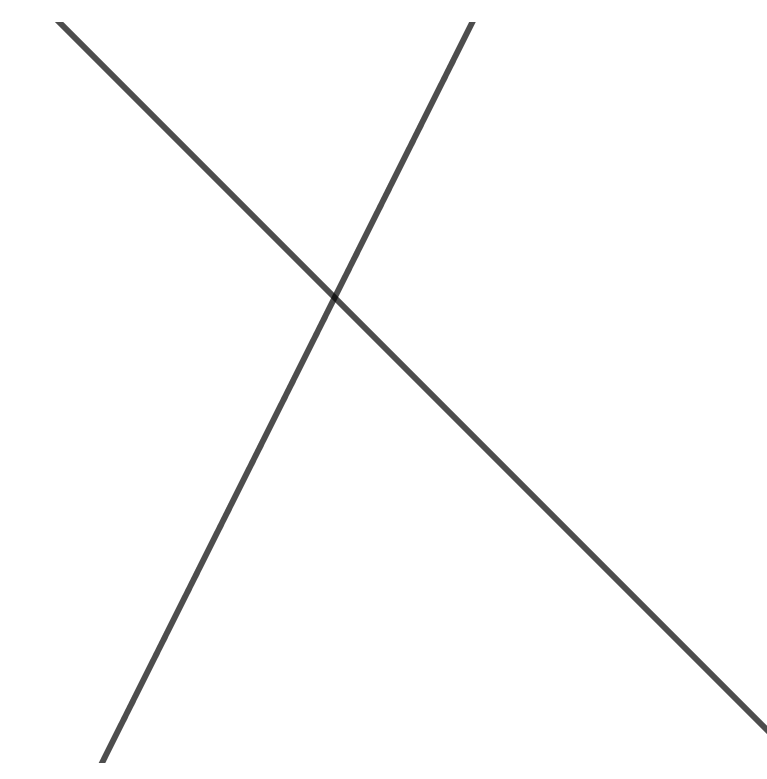
\includegraphics[width=0.12\textwidth]{twolines_3}}
\\\hline
\(m=m'\), \(n=n'\) & \(m=m'\), \(n\neq n'\) & \(m\neq m'\)
\\\hline
$\frac{a}{a'}=\frac{b}{b'}=\frac{c}{c'}$
 & $\frac{a}{a'}=\frac{b}{b'}\neq\frac{c}{c'}$
 & $\frac{a}{a'}\neq\frac{b}{b'}$
\\\bottomrule
\end{tabu}
\item
세 가지 공식
\begin{itemize}
\item
\(y=m(x-x_1)+y_1\)
\item
\(y=\frac{y_2-y_1}{x_2-x_1}(x-x_1)+y_1\)
\item
\(\frac xa+\frac yb=1\)
\end{itemize}
\item
두 직선의 교점을 지나는 직선
\[(ax+by+c)+m(a'x+b'y+c')=0\]
\item
점과 직선 사이의 거리
\[d=\frac{|ax_1+by_1+c|}{\sqrt{a^2+b^2}}\]
\end{enumerate}
\end{document}